\documentclass[a4paper,twocolumn]{article}
\usepackage[a4paper,top=1cm,bottom=1cm,left=1cm,right=1cm]{geometry}
\usepackage[T1]{fontenc}
\usepackage[utf8]{inputenc}
\usepackage[italian]{babel}
\usepackage{amsmath}
\usepackage{float}
\usepackage{xcolor}
\usepackage{hyperref}
\usepackage{caption}
\usepackage{subcaption}     %subfigure
\usepackage{float}
							%disegni
\usepackage{graphicx}
\usepackage{tikz}
							%unità di misura
\usepackage{SIunits}
							%tabelle di grandezza x
\usepackage{tabularx}
							%generalità testo
\title{Time of flight}
\author{Andrea Foresi}
\date{\today}

\begin{document}
\maketitle

\begin{abstract}
Scopo di questa esperienza è quello di misurare la distribuzione della velocità dei raggi cosmici, muoni, che raggiungono la superficie terrestre e valutare quale frazione di essi sia relativistica. Oltre a questa misura si mostrano la velocità della luce nella barra scintillante (\ref{sec:VLuce}), l'attenuazione dei segnali luminosi nello scintillatore (\ref{sec:AttPos}), la dipendenza del segnale impulsivo dall'angolo di incidenza dei muoni sulla barra (\ref{sec:Angolo}).
\end{abstract}

\tableofcontents


\section{Apparato sperimentale}
\label{sec:AppSper}
\begin{itemize}
\item Barra scintillante BICRON BC408 con 2 fotomoltiplicatori alle estremità (numeri 1 e 2).
\item Scintillatore plastico piano mobile di piccole dimensioni con relativo PMT (numero 3).
\item Scintillatore plastico piano di grandi dimensioni con relativo PMT (numero 4).
\item Strumentazione DAQ:
\begin{itemize}
\item Oscilloscopio 4 canali Tektronix MDO34.
\item Alimentatore 4 canali CAEN DT5533E.
\item Moduli NIM: ADC converter CAEN N6725S, discriminatore, contatore.
\end{itemize}
\end{itemize}

\begin{figure}[H]
    \centering
    \title{Apparato Sperimentale}
\begin{center}
\begin{tikzpicture}[scale=0.6]

\draw[gray, very thick] (0,12) rectangle (12,12.1);
\draw (1,12.5) node[left] {PMT\#1};
\draw(11,12.5) node[right] {PMT\#2};
\filldraw[color=black!60, fill=black!50, very thick] (0,12) rectangle (1,12.1);
\filldraw[color=black!60, fill=black!50, very thick] (11,12) rectangle (12,12.1);
\draw[<->] (6,12.4) -- (10.75,12.4);
\draw(3,12.6) node {$140\:$\centi\metre};
\draw[<->] (1.25,12.4) -- (6,12.4);
\draw(9,12.6) node {$140\:$\centi\metre};
\draw[<->](-0.2,12) --(-0.2,2);
\draw(-0.5,7) node[left,rotate=90] {$h\:=\:176\:$\centi\metre};
\draw[dotted](6,13) -- (6,-1);
\draw[->,dotted,color=red] (10,13) -- (4.95,-1);
\draw[<->](9.8,11.9)--(6.27,2.1);
\draw[<->](6,11.8)--(9.65,11.8);
\draw(8.1,6.5) node[rotate=64,right] {d};
\draw(8,11.65) node {$x$};

\draw(6,4) [right]node{$\theta$};

\filldraw[color=black!60, fill=black!50, very thick] (6,2) circle (0.1);
\draw[gray, very thick] (5.5,2.05) rectangle (6.5,1.95);
\draw(2.5,2) node[right] {PMT-3};
\draw[color=black!60,fill=black!50,very thick] (3.5,1.05) rectangle (8.5,0.95);
\draw (1,1) node {lastra/e di piombo};
\draw[gray, very thick] (3.5,0.05) rectangle (8.5,-0.05);
\filldraw[color=black!60, fill=black!50, very thick] (2.5,0.05) rectangle (3.5,-0.05);
\draw(2.5,0) node[left] {PMT-4};

\draw(0.8,-3) node{PMT-3};
\draw(2,-3)--(3,-3)--(3,-5.5)--(2.5,-6)--(2,-5.5)--(2,-3);
\draw[<->](3.3,-3)--(3.3,-5.5);
\draw[<->](2,-2.7)--(3,-2.7);
\draw(3.5,-4.5) node[rotate=90] {$40\:$\centi\metre};
\draw(2.5,-2.5) node{$ 22\:$\centi\metre};
\filldraw[color=black!60, fill=black!50, very thick] (2.45,-6) rectangle (2.55,-7);

\draw(5.8,-3) node{PMT-4};
\draw(7,-3)--(9,-3)--(9,-5.5)--(8,-6)--(7,-5.5)--(7,-3);
\draw[<->](9.3,-3)--(9.3,-5.5);
\draw[<->](7,-2.7)--(9,-2.7);
\draw(9.5,-4.5) node[rotate=90] {$51\:$\centi\metre};
\draw(8,-2.5) node{$40\:$\centi\metre};
\filldraw[color=black!60, fill=black!50, very thick] (7.95,-6) rectangle (8.05,-7);

\end{tikzpicture}
\caption{la linea rossa tratteggiata indica una traiettoria di una qualsiasi particella passante per il sistema. Con x è indicata la posizione nella quale la particella passa attraverso la barra.}
\label{fig:AppSperSschema}
\end{center}
\end{figure}

Il PMT-3 mobile è posizionabile tramite delle guide, sia sopra la barra scintillante lunga, che sopra lo scintillatore numero 4, come si vede in figura \ref{fig:PMT3posPMT4}.

\paragraph{Misure preliminari}
\begin{itemize}
\item h\;=\;176,0\,$\pm$\,0,5\:\centi\metre
\item L\;$\sim$\;280\:\centi\metre, lunghezza barra scintillante
\item PMT-3: 40,0\,$\pm$\,0,2\:\centi\metre\;x\;22,0\,$\pm$\,0,2\:\centi\metre 
\item PMT-4: 51,0\,$\pm$\,0,2\:\centi\metre\;x\;40,0\,$\pm$\,0,2\:\centi\metre 
\item Barra scintillante $\sim$ 2,80\:\metre\;x\;4\:\centi\metre\;x\;4\:\centi\metre, indice di rifrazione $n\sim\:1,58$\footnote{Per le misure di grandezze sono state riportate quelle segnate del datasheet, in quanto essendo già interamente ricoperta la barra dalle protezioni non è stato possibile effettuare delle misure precise di controllo. Altri dati sono visionabili sul sito \url{https://www.crystals.saint-gobain.com/sites/imdf.crystals.com/files/documents/bc400-404-408-412-416-data-sheet.pdf}}.
\item Altezza del PMT-3 rispetto al PMT-4 $\sim$\:3\,\centi\metre\;($<<$h).
\end{itemize}

\paragraph{Caratteristiche ADC}
Di seguito sono elencate le caratteristiche principali, alcune delle quali hanno influenzato maggiormente i risultati dell'esperienza\footnote{Per altre caratteristiche il datasheet è scaricabile al link \url{https://www.caen.it/products/n6725/}, previa iscrizione al sito.}:
\begin{itemize}
\item 8 canali analogici
\item Rate campionamento 250\,MS\per\second, cioè 1 campione ogni 4\,\nano\second
\item Record Length 1030\,campioni, 4120\,\nano\second
\item Risoluzione 14\,bit
\end{itemize}

\subsection{Funzionamento in breve}
Una particella che attraversa la barra scintillante lunga può essere rivelata da entrambi i PMT installati ai capi di essa. La differenza tra gli istanti di tempo di rivelazione dei segnali può diventare una misura utile a ricavare la posizione per la quale è passata la particella. Per il tempo di volo si prenderà un intervallo di tempo tra i PMT-1 o PMT-2 con il PMT-3 posizionato in basso, ad un'altezza h rispetto alla barra lunga. Con queste misure sarà possibile ricavare $v=\frac{\textnormal{x}}{\textnormal{TOF}}$.\\
Inoltre la carica rilasciata dai segnali, letta tramite strumentazione DAQ, che sappiamo essere legata da leggi di proporzione diretta alla velocità e quindi all'energia della particella, può essere una misura per l'energia rilasciata dalla particella nella barra.

\section{Calibrazione app. sperimentale}
Per prima cosa sono stati scelti i punti di lavoro dei 4 PMT.\\
Dopo aver discriminato il segnale dal rumore (sec\,\ref{sec:DiscrSegn}), in un primo momento sono stati calibrati i fotomoltiplicatori, osservando il comportamento del rate di eventi in singola rivelati in funzione della tensione di alimentazione applicata ai capi dei PMT (sec\,\ref{sec:CalSin}).\\
Infine, si è proceduti con la scelta dell'alimentazione tramite misura del rapporto tra coincidenze doppie e coincidenze triple\footnote{Le coincidenze verranno indicate con la simbologia C$_{ijk}$, nella quale i,j,k indicano il numero dei PMT messi in coincidenza. Per esempio C$_{12}$ indica una coincidenza doppia tra i PMT-1 e PMT-2, mentre C$_{123}$ indica una coincidenza tripla tra i PMT-1, PMT-2 e PMT-3.} (sec\,\ref{sec:Coinc}).

\subsection*{Errori stabilità}
\label{sec:ErrSis}
Nel corso dell'esperienza sono stati evidenziati alcuni errori di stabilità della strumentazione.
Di seguito, li elenchiamo una sola volta, per non appesantire troppo la lettura:
\begin{itemize}
\item Su tutte le soglie impostate con il modulo NIM discriminatore si deve applicare un errore di circa $\pm$\,2\:\milli\volt\;, in quanto da un'accensione all'altra si venivano a creare delle discrepanze di pochi \milli\volt\;sulla soglia di discriminazione dei segnali che non è stata verificata costantemente durante il corso dell'esperienza. Quindi, per esempio una misura di soglia come -50\:\milli\volt\;va letta come: 50\,$\pm$\,2\:\milli\volt.
\item Tutte le volte che si è impostata un'alimentazione su un particolare fotomoltiplicatore tramite alimentatore CAEN DT5533E, si è notata da monitor una discrepanza tra il valore impostato e quello effettivamente letto di 0,2-0,3\:\volt. Perciò, le misure che verranno indicate con 1600\,\volt\; andranno lette come 1600,0\,$\pm\,$0,3\:\volt.
\end{itemize}

\subsection{Discriminazione}
\label{sec:DiscrSegn}
Per questa discriminazione sono stati osservati dei segnali tramite oscilloscopio, come quelli in figura\,\ref{fig:SegnaliOsc}.

\begin{figure}[ht]
\centering
\title{Segnali su oscilloscopio}
\begin{center}
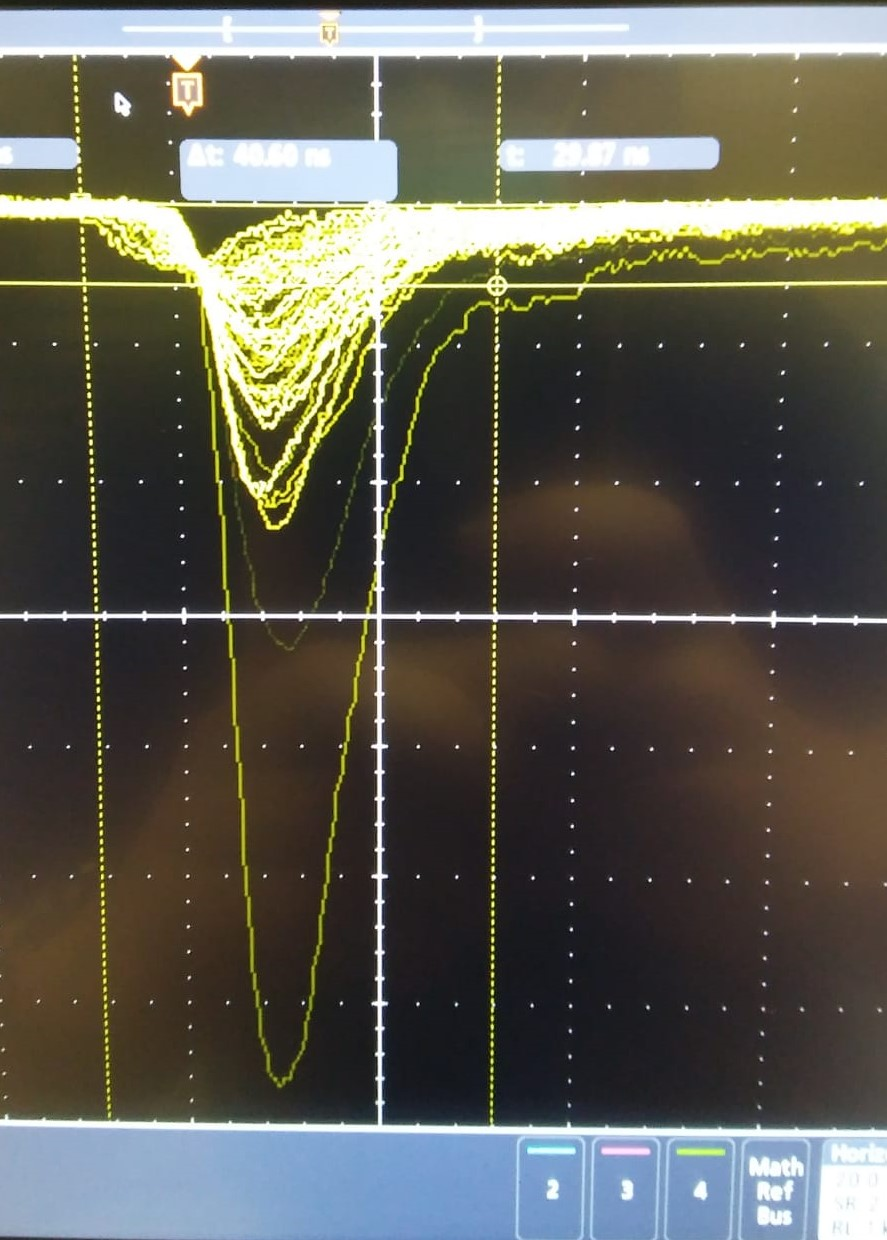
\includegraphics[width=0.25\textwidth]{./immagini/TimeOfFlight/SegnaliOsc.jpg}
\caption{Divisioni: 10\:ns\per div nei tempi; 20\:mV/div per i voltaggi}
\label{fig:SegnaliOsc}
\end{center}
\end{figure}

La scelta del tempo di lunghezza del segnale output del discriminatore è stata fatta con l'osservazione della durata dei tempi di un singolo impulso ($\sim$\:15-20\:\nano\second\;come da figura\,\ref{fig:SegnaliOsc}), al quale però è stato pensato di aggiungere un possibile ritardo, dovuto alla differenza di trasmissione. Infatti, dovendo misurare dei ritardi di qualche ns tra due o più segnali, sono stati stimati due tempi di percorrenza, uno riferito alle particelle e uno ai segnali impulsivi:

\begin{itemize}
\item Il primo ritardo è dovuto alla velocità della luce nella barra scintillante lunga: $v_{\textnormal{teorica}}$ = $\frac{30}{\textnormal{n}} \, \frac{\textnormal{cm}}{\textnormal{ns}} \; \simeq \; 19 \,\frac{\centi\metre}{\textnormal{ns}}$, dove n è l'indice di rifrazione della barra scintillante. Perciò si ha un ritardo massimo di $\frac{L \; = \; 280 \, \textnormal{cm}}{v \; = \; 19\, \frac{\textnormal{cm}}{\textnormal{ns}}} \; \simeq \; 15\,\nano\second$.
\item Il secondo ritardo è quello dovuto al tempo di volo delle particelle (TOF). La distanza massima che percorrono le particelle è di circa: $d = \sqrt{(\frac{L}{2})^2 + h^2} \simeq 224$\,cm, e supponendo una velocità di $10\,\frac{\textnormal{cm}}{\textnormal{ns}}$, si ottiene un ritardo di $\sim 21$\,ns.
\end{itemize}

Perciò, dopo aver visualizzato segnali come quelli di figura\,\ref{fig:SegnaliOsc}, sono stati scelti i seguenti livelli per discriminare i segnali che raggiungono i PMT:

\begin{itemize}
\item -45\,mv di threshold.
\item 50\,ns di durata del segnale discriminato.
\end{itemize}

\subsection{Conteggi in singola}
\label{sec:CalSin}
Per quanto riguarda l'osservazione dei conteggi in singola sono state riprodotte le curve "Conteggi vs V$_{Alim}$" dei PMT-1 e PMT-3.

\begin{figure}[H]
\centering
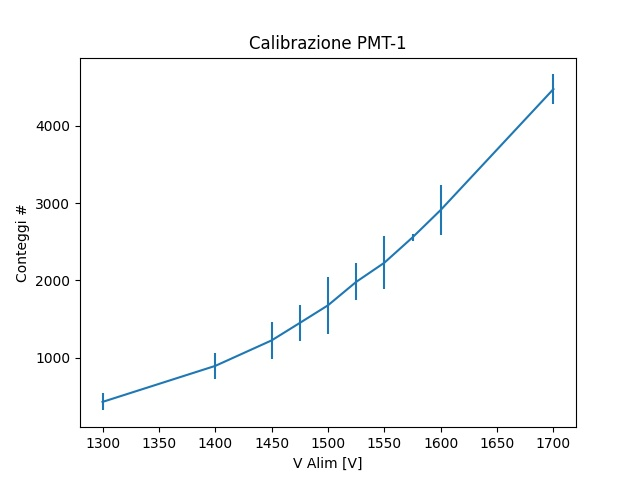
\includegraphics[width=0.45\textwidth]{./immagini/TimeOfFlight/CalSinPMT-1.jpg}
\caption{Gli errori in figura sono moltiplicati per 10.}
\label{fig:CalSinPMT-1}
\end{figure}

\begin{figure}[H]
\centering
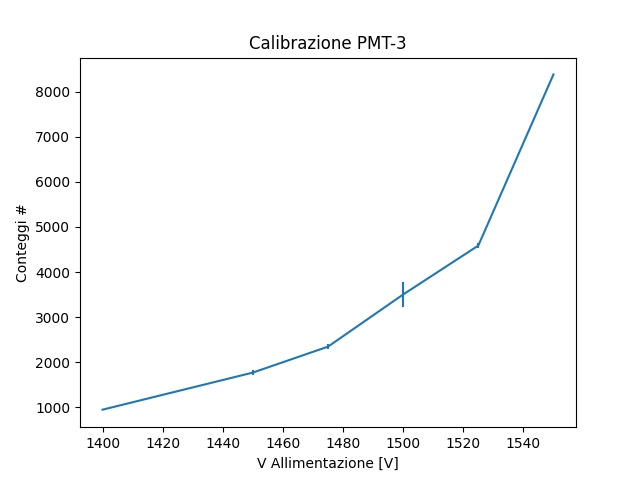
\includegraphics[width=0.45\textwidth]{./immagini/TimeOfFlight/CalSinPMT-3}
\caption{}
\label{fig:CalSinPMT-3}
\end{figure}

Per ogni tensione di alimentazione impostata sono stati presi per diverse volte conteggi per una durata di 10 secondi. L'errore associato è dunque una semplice devstd delle misure dei conteggi prese.\\
Non si evidenzia un plateau in nessuno dei due grafici in figure\,\ref{fig:CalSinPMT-1} e \ref{fig:CalSinPMT-3}, perciò si sceglie di fissare inizialmente le alimentazioni di tutti i PMT (PMT-2 compreso) a 1600\,V.

\subsection{Coincidenze}
\label{sec:Coinc}
Per la calibrazione tramite coincidenze sono state fatte due prove: la prima ricercando un plateau nel rapporto tra coincidenze doppie/triple (sec\,\ref{sec:CoincPla}), la seconda, invece, andando a massimizzare l'efficienza, controllando che i conteggi in singola non aumentassero di troppi ordini di grandezza (sec\,\ref{sec:CoincMax}).\\
Inoltre, è stata controllata un'eventuale dipendenza dell'efficienza in funzione della soglia impostata sul discriminatore.\\
Per le calibrazioni dei PMT-1 e PMT-2 è stato tenuto lo scintillatore numero 3 sopra il centro della barra scintillante lunga.

\begin{figure}
\centering
\title{Coincidenze su oscilloscopio}
\begin{center}
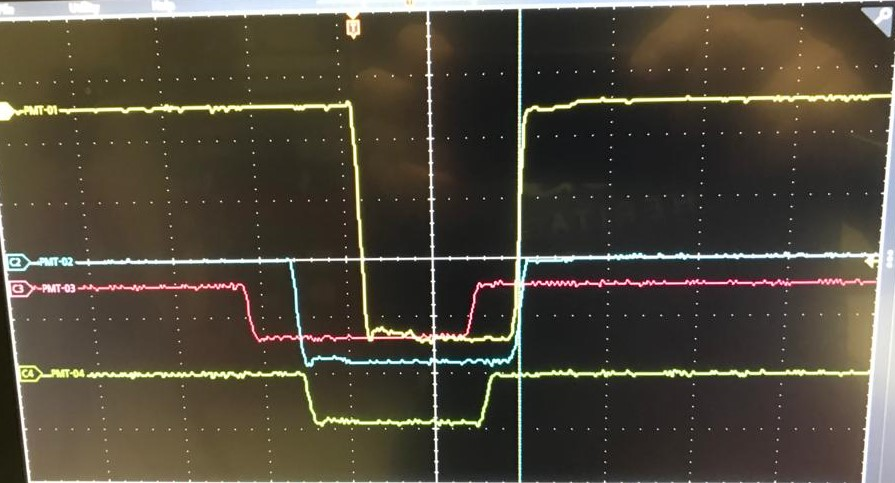
\includegraphics[scale=0.35]{./immagini/TimeOfFlight/CoincOscill.jpg}
\caption{In giallo il segnale della coincidenza tripla. Verde e blu PMT collegati alla barra scintillante. Rosso PMT-3. Trigger impostato sulla coincidenza tripla.}
\label{fig:ExCoinc}
\end{center}
\end{figure}

\subsubsection{Ricerca plateau}
\label{sec:CoincPla}
Per primo è stato calibrato il PMT-1 dove, le coincidenze doppie sono C$_{23}$ e quelle triple C$_{123}$, le alimentazioni dei PMT sono $V_{Alim2}\:=\:V_{Alim3}\:=\:1600$\,V e V$_{Alim1}$ variabile, le soglie del discriminatore impostate a -45\,mV per i PMT 1 e 2 e -50\,mV per il PMT-3.

\subsubsection*{Distribuzione Binomiale}
\label{sec:DistrBino}
Le misure di efficienza, che vedremo più avanti, seguono una distribuzione binomiale, il cui errore su una misura di $\epsilon$ è data da $\sigma =\sqrt{\frac{\epsilon(1-\epsilon)}{N}}$, dove $\epsilon\:=\:\frac{n}{N}$, n è il numero di occorrenze positive e N quello totale. Nel caso di $\epsilon$\:=\:1, invece, associamo alla misura un errore pari a $\epsilon_{90\%} = (1-0,90)^{\frac{1}{N+1}}$, dove si è fissato un livello di confidenza del 90$\%$ sulla correttezza della misura di $\epsilon$.

\begin{figure}[H]
\centering
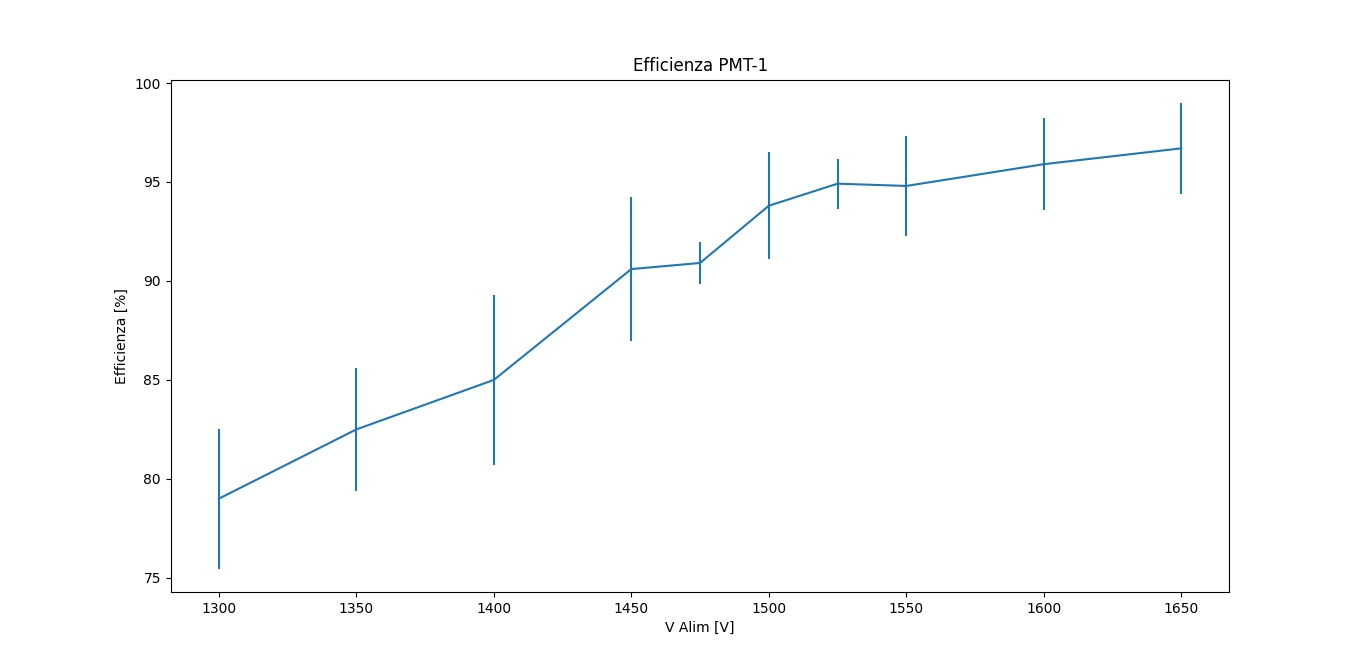
\includegraphics[width=0.45\textwidth]{./immagini/TimeOfFlight/EffPMT145mV}
\caption{Si è deciso di selezionare una tensione di poco superiore a quella che sembra corrispondere ad un plateau nelle coincidenze.}
\label{fig:EffPMT145mV}
\end{figure}

Osservando la figura\,\ref{fig:EffPMT145mV}, per il PMT-1 si potrebbe selezionare un'alimentazione di 1510\,V corrispondente ad un'efficienza del 93.8$\%$.\\
Questa scelta, però, può risultare limitante; infatti, facendo una stima della probabilità di avere coincidenze casuali aumentando l'alimentazione, si nota che, anche portando il fotomoltiplicatore ad avere un'efficienza, ritenuta alta, del 96$\%$, questa rimane molto bassa. Perciò, si è pensato fosse possibile cercare un'alimentazione, che aumentasse l'efficienza del rivelatore fino ad un minimo del 98$\%$, sempre che questa alimentazione non facesse aumentare considerevolmente il numero di coincidenze casuali.

\paragraph{Coincidenze casuali}
Nel caso di una coincidenza tripla, consideriamo $f_i$ come i conteggi per secondo di un singolo PMT-i e $\tau_i$ la lunghezza del segnale discriminato del PMT-i. Perciò, una coincidenza tra 3 canali a meno di costanti nel nostro caso vale circa:

\begin{center}
$f_{cas} = f_1 \cdot f_2 \cdot f_3 \cdot \tau _1 \cdot \tau _2 \simeq (5\usk10^2)\,\textnormal{cps} \cdot (5\usk 10^2)\,\textnormal{cps} \cdot 10^3\,\textnormal{cps} \cdot (50\usk10^{-9})^2\,\nano\square\second = 6,25\usk10^{-7} \textnormal{cps}$
\end{center}

dove abbiamo considerato $\tau_1 = \tau_2$, perché entrambi di 50\,\nano\second. Le $f_i$ corrispondono ai conteggi al secondo del PMT-i con le alimentazioni indicate all'inizio del paragrafo\,\ref{sec:CoincPla} e V$_{Alim1}$ = 1510\,\volt. 

\subsubsection{Massimizzazione dell'efficienza}
\label{sec:CoincMax}
Considerando le stesse coincidenze della sezione precedente (\ref{sec:CoincPla}), si cerca per i PMT una tensione di alimentazione, che corrisponda ad un'efficienza minima del 98$\%$.

\paragraph{PMT-2, scelta soglia discriminazione}
Per la prima calibrazione, quella del PMT-2, è stata effettuata una prova per la dipendenza della curva di efficienza dal valore di soglia impostato con il modulo discriminatore NIM. Sono così state riprodotte due curve di efficienza con due livelli di soglia differenti.

\begin{figure}[H]
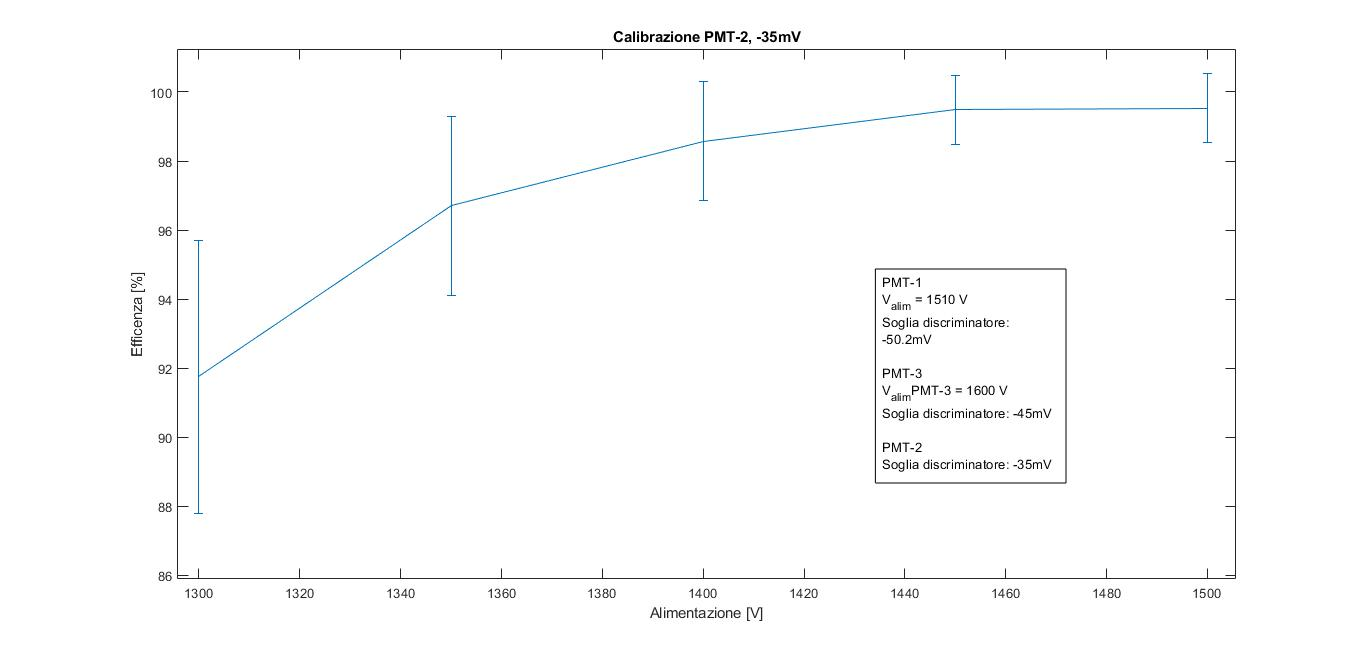
\includegraphics[width=0.45\textwidth]{./immagini/TimeOfFlight/EffPMT235mV.jpg}
\caption{Soglia -35\,mV}
\label{fig:EffPMT235mV}
\end{figure}
\begin{figure}[H]
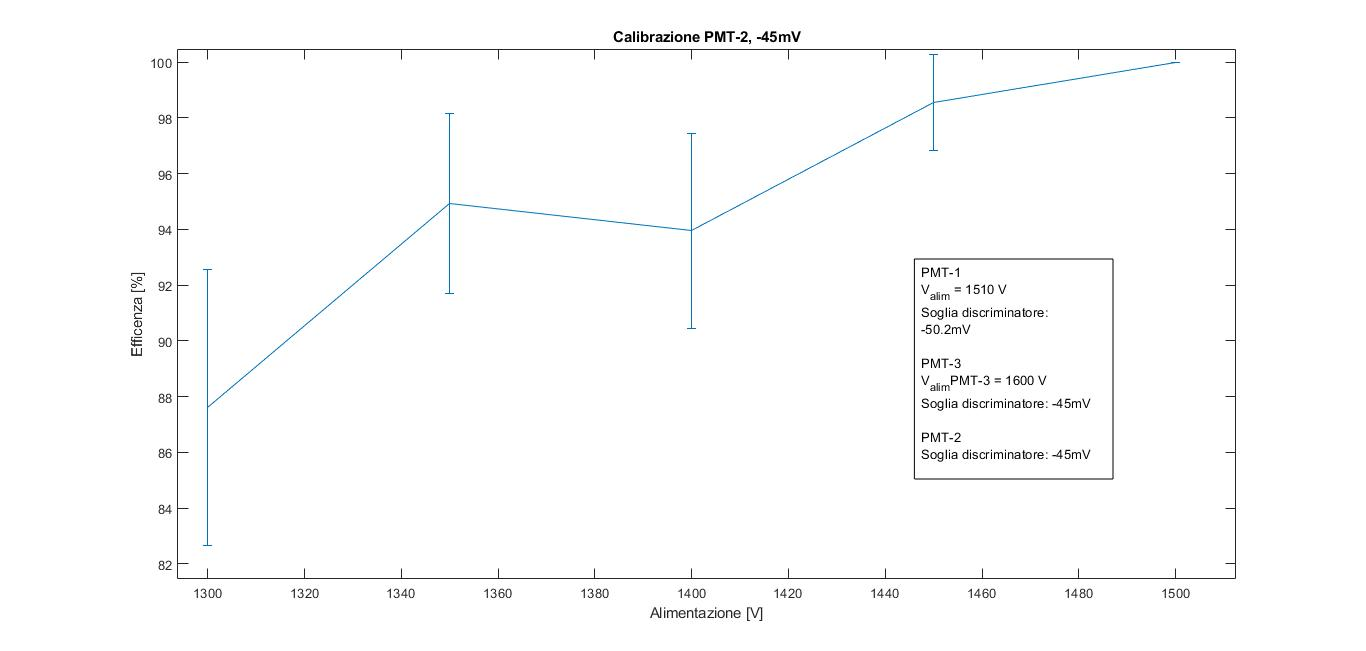
\includegraphics[width=0.45\textwidth]{./immagini/TimeOfFlight/EffPMT245mV.jpg}
\caption{Soglia -45\,mV}
\label{fig:EffPMT245mV}
\end{figure}

Nei tentativi a soglie diverse si nota che, quando si raggiunge l'efficienza desiderata del 98$\%$, si hanno i seguenti conteggi in singola:

\begin{table}[H]
\begin{tabular}{|c|c|c|c|}
\hline
Soglia [mV] & V$_{Alim}$ [V] & PMT-1 [cps] & PMT-2 [cps] \\
\hline
-35 & 1400 & 149 & 142\\
-45 & 1450 & 150 & 142\\
\hline
\hline
Soglia [mV] & V$_{Alim}$ [V] & PMT-3 [cps] &   \\
\hline
-35 & 1400 & 986 &\\
-45 & 1450 & 852 &\\
\hline
\end{tabular}
\caption{}
\end{table}

Non essendoci differenze sostanziali, è stata preferita la scelta con:

\begin{center}
soglia = -35\,mV; V$_{Alim_2}$\:=\:1400\,V.
\end{center}

Perciò, tutti i segnali dei 4 PMT sono stati discriminati con un threshold uguale al PMT-2, soglia = -35\,mV.


\paragraph{PMT-1}
Per il PMT-1 le coincidenze doppie sono C$_{23}$ e le triple C$_{123}$. Il PMT-3 è sempre posizionato sopra il centro della barra scintillante lunga.

\begin{figure}[H]
\centering
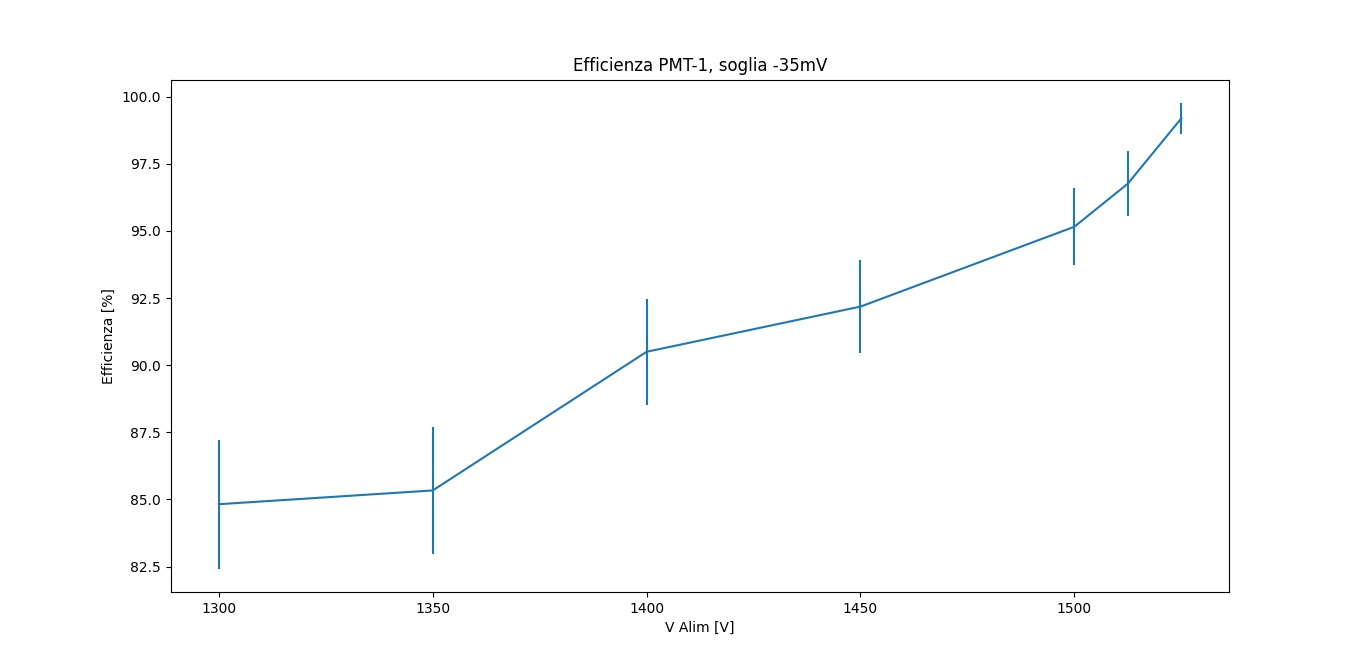
\includegraphics[width=0.45\textwidth]{./immagini/TimeOfFlight/EffPMT135mV}
\caption{Per un valore di alimentazione $\geq$\:1550\,V sono state trovate un numero maggiore di triple rispetto alle doppie. V$_{Alim_3}$\:=\:1600\,V, V$_{Alim_2}$\:=\:1400\,V.}
\label{fig:EffPMT135mV}
\end{figure}

Facendo riferimento alla figura\,\ref{fig:EffPMT135mV}, è stato deciso di alimentare il PMT-1 con V$_{Alim_1}$\:=\:1525\,V.

\paragraph{PMT-3}
Il PMT-3 è stato alimentato e discriminato come il PMT-2.

\paragraph{PMT-4}
\label{sec:CalPMT-4}
Per questa calibrazione abbiamo posizionato lo scintillatore 3 esattamente sopra lo scintillatore 4 come in figura\,\ref{fig:PMT3posPMT4}.\\
Le doppie sono C$_{23}$ e le triple C$_{234}$.

\begin{figure}[H]
\centering
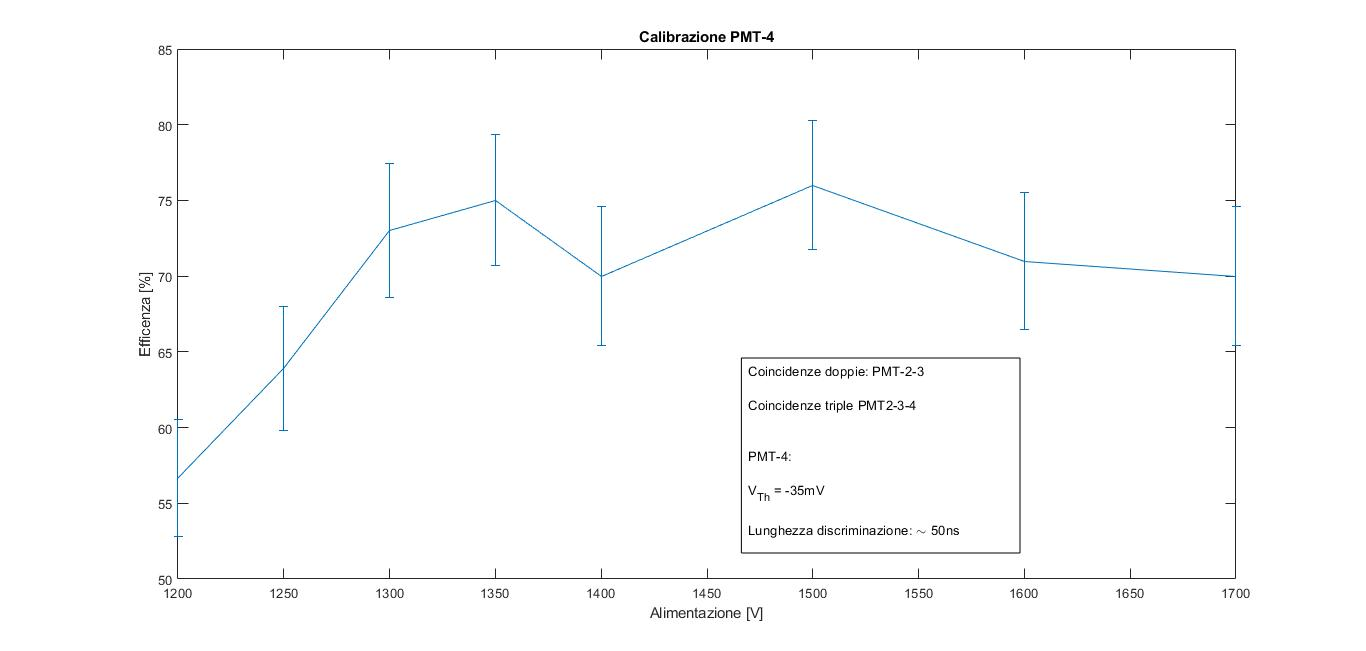
\includegraphics[width=0.45\textwidth]{./immagini/TimeOfFlight/CoincidenzePMT4.jpg}
\caption{I segnali del PMT-4 sono stati discriminati con una soglia a -35\,mV e una lunghezza del segnale discriminato di 50\,ns, proprio come per tutti gli altri PMT.}
\label{fig:EffPMT4}
\end{figure}

Notiamo che, nonostante lo scintillatore 4 sia notevolmente più grande del 3, l'efficienza è ben diversa da quella attesa, tendente al 100$\%$ con l'aumentare dell'alimentazione del PMT-4, ma si stabilizza all'incirca sul 70$\%$.

\begin{figure}[ht]
\centering
\title{Posizione PMT-3 e PMT-4}
\begin{center}
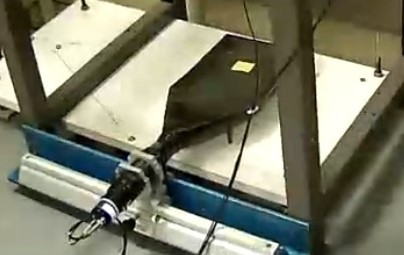
\includegraphics[scale=0.4]{./immagini/TimeOfFlight/CalPMT4app.jpg}
\caption{Lo scintillatore 4 è posto sotto del legno, ne è purtroppo poco visibile solo il perimetro segnato a matita.}
\label{fig:PMT3posPMT4}
\end{center}
\end{figure}

I problemi potrebbero essere dovuti a parti elettroniche, connessioni o ad effetti fisici, non sicuramente geometrici.\\
La scelta per l'alimentazione del PMT-4 è stata presa optando per un valore di alimentazione che si avvicinasse ai fotomoltiplicatori precedenti, e che presentasse conteggi in singola dell'ordine del centinaio di Hz:

\begin{table}[H]
\begin{flushleft}
\begin{tabular}{|c|c|c|c|}
\hline
V$_{Alim} [V]$ & doppie & triple & PMT-1 \\
\hline
1400 & 100 & 84 & 668883 \\
\hline
1350 & 100 & 67 & 62857 \\
\hline
\hline
 PMT-2 &  PMT-3 &  PMT-4 & Tempo [ms]\\
\hline
48185 & 135507 & 92826 & 273037\\
\hline
41377 & 168528 & 86412 & 349377\\
\hline
\end{tabular}
\end{flushleft}
\caption{Sono indicati i conteggi in singola dei PMT, dopo aver trovato 100 doppie. Il tempo corrisponde al tempo impiegato per rivelare 100 doppie.}
\end{table}

In entrambi i casi si rimane su valori delle centinaia di cps. Si sceglie di alimentare con 1400\,V con $\sim$\:340\,cps.



\section{Velocità della luce nella barra scintillante}
\label{sec:VLuce}
\subsection{Cenni teorici}
Ogni volta che una particella carica attraversa la barra scintillante, questa perde energia per ionizzazione nel mezzo, e la quantità di energia persa segue l'andamento della nota curva Bethe-Block.\\
Successivamente, per diseccitamento vengono emessi fotoni, come scintille, la cui luminosità è una funzione dell'energia persa per unità di lunghezza\footnote{La luminosità segue la legge di Birks: $\frac{dL}{dx} = \frac{A\frac{dE}{dx}}{1+\textnormal{kB}\frac{dE}{dx}}$, dove kB è una costante sperimentale. La legge ha una dipendenza direttamente proporzionale tra la luminosità ($\frac{dL}{dx}$) e l'energia persa ($\frac{dE}{dx}$), fino a quando non raggiunge un massimo sul quale si stabilizza.}.\\
I fotoni, non essendo nel vuoto, viaggeranno ad una velocità ridotta del valore dell'indice di rifrazione del materiale (n $\simeq$ 1,58). Dunque $v_{luce} = \frac{30\frac{\centi\metre}{\nano\second}}{1,58} \simeq 19,0 \frac{\centi\metre}{\nano\second}$.

\subsection{Misure}
Per misurare questa velocità si è posizionato il PMT-3 in diversi punti sopra la barra scintillante lunga, così da fissare la distanza percorsa dalla luce verso un PMT, a meno di un errore dovuto alla larghezza dello scintillatore (vedi paragrafo\,\ref{sec:ErrPosX}).\\
Per associare la velocità dei fotoni ai $\Delta t$ misurabili tramite strumentazione DAQ, è stata utilizzata la seguente formula:

\begin{equation}
\Delta t_{21} = \frac{\textnormal{2\usk x - L}}{v_{luce}} + (\tau_1 - \tau_2)
\label{equ:VLuceBarra}
\end{equation}

dove L è la lunghezza della barra; $\Delta t_{21}$ è il ritardo tra i segnali provenienti dai PMT 1 e 2 (quelli collegati alle estremità della barra); x è la posizione che scegliamo in base a dove poniamo il PMT-3; $\tau_1$ e $\tau_2$ sono dei possibili ritardi tra le trasmissioni dei segnali, che vanno ad influire unicamente sull'offset della retta; infine, l'inverso del coefficiente angolare (\textit{v$_{luce}$}) sarà la nostra velocità.\\
La misura dei ritardi tra i segnali impulsivi è stata eseguita in due maniere, sia utilizzando direttamente una funzione dell'oscilloscopio sia utilizzando l'ADC converter.\\
Il trigger è impostato per entrambe le misure sulla coincidenza tripla C$_{123}$.

\subsubsection{Analisi dati tramite oscilloscopio}
\label{sec:VBarOsc}
Sono stati presi 100 eventi per ognuna delle posizioni scelte e ne è stata misurata media e devstd con l'oscilloscopio stesso. Quindi ne è stato fatto un fit con la retta in equazione \ref{equ:VLuceBarra}.

\begin{figure}[H]
     \centering
     \begin{subfigure}[b]{0.47\textwidth}
         \centering
         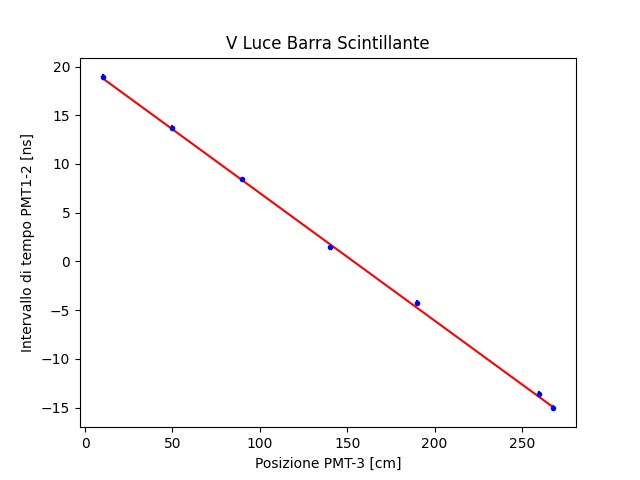
\includegraphics[width=\textwidth]{./immagini/TimeOfFlight/VLightBarra.jpg}
         \caption{In rosso la retta di fit}
         \label{fig:FitVLightBarra}
     \end{subfigure}
     \hfill
     \begin{subfigure}[b]{0.47\textwidth}
         \centering
         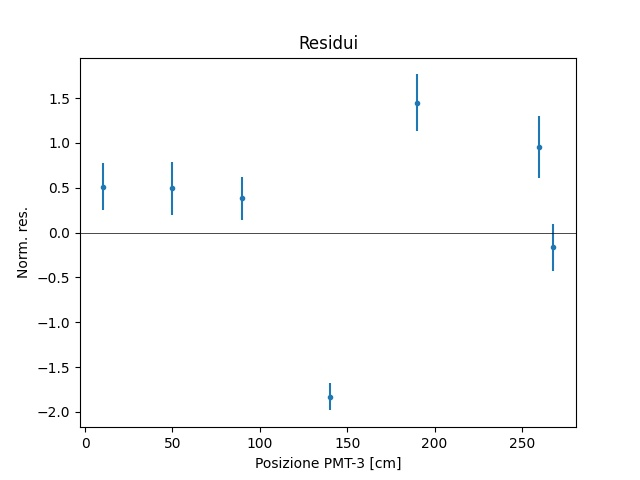
\includegraphics[width=\textwidth]{./immagini/TimeOfFlight/ResVLightBarra.jpg}
         \caption{}
         \label{fig:ResVLIghtBarra}
     \end{subfigure}
     \caption{Gli errori sono la devstd delle misure divise per 10 (radice del numero di eventi presi).} 
     \label{fig:FitLinVLightBarra}
\end{figure}

Dal fit sono stati ottenuti i seguenti risultati:

\begin{table}[H]
\begin{tabular}{|c|c|c|c|c|}
\hline
$v_{luce}$ [$\frac{\centi\metre}{\nano\second}$] & off [ns] & $\chi ^2$ & ndof & norm.cov. \\
\hline
-15,28 $\pm$ 0,16 & 20,10 $\pm$ 0,22& 7,04 & 5 & 0,86\\
\hline
\end{tabular}
\caption{}
\label{tab:ResFitVLOsc}
\end{table}

Il segno meno è dovuto alla scelta della differenza tra i PMT-1 e PMT-2.

\subsubsection{Analisi dati ADC}
\label{sec:VBarADC}
Per questa analisi abbiamo preso diversi segnali in coincidenza tra PMT 1, 2 e 3, con il PMT-3 posizionato in alcune posizioni della barra come nel caso precedente, e calcolato media e devstd dei $\Delta t$ ricavati.

\begin{figure}[H]
     \begin{subfigure}[b]{0.47\textwidth}
         \centering
         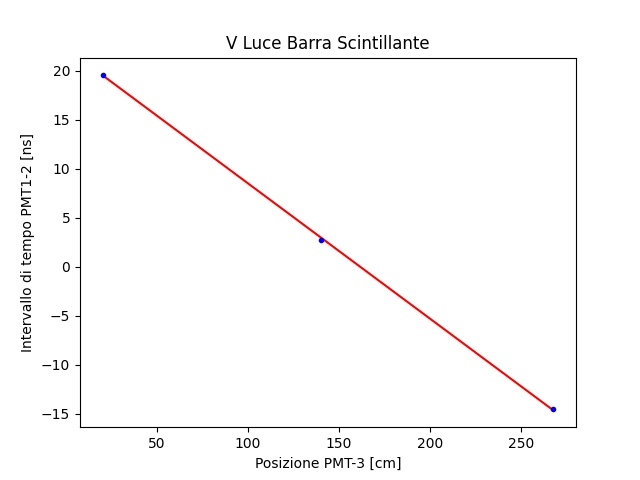
\includegraphics[width=\textwidth]{./immagini/TimeOfFlight/VLightBarraADC}
         \caption{}
         \label{fig:FitVLightBarraADC}
     \end{subfigure}
     \hfill
     \begin{subfigure}[b]{0.47\textwidth}
         \centering
         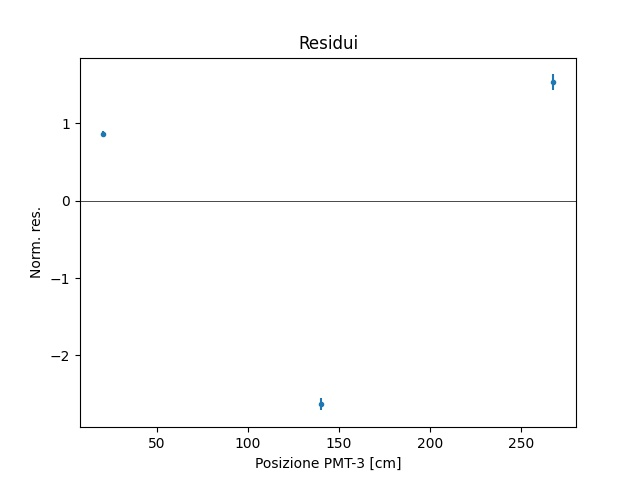
\includegraphics[width=\textwidth]{./immagini/TimeOfFlight/ResVLightBarraADC}
         \caption{}
         \label{fig:ResVLIghtBarraADC}
     \end{subfigure}
     \caption{}        
     \label{fig:FitLinVLightBarraADC}
\end{figure}

Dal fit abbiamo ottenuto i seguenti risultati:

\begin{table}[H]
\begin{tabular}{|c|c|c|c|c|}
\hline
v$_{luce}$ [$\frac{\centi\metre}{\nano\second}$] & off [ns] & $\chi ^2$ & ndof & norm.cov.  \\
\hline
-14,48 $\pm$ 0,15 & 22,33 $\pm$ 0,02 & 12,61 & 1 & 0,64\\
\hline
\end{tabular}
\caption{}
\label{tab:ResFitVLADC}
\end{table}

\subsection{Risultati}
In entrambi i casi la velocità è risultata inferiore a quella attesa ($\sim$\:19\,$\frac{\centi\metre}{\nano\second}$), probabilmente perché i fotoni non compiono delle traiettorie lineari dal punto in cui vengono emessi fino al fotocatodo, ma, riflettendosi lungo le pareti della barra scintillante, compiono un tragitto più lungo.\\
Nella misura con l'ADC sono stati presi troppo pochi dati. Ciò si evince dal rapporto $\frac{\chi^2}{\textnormal{ndof}}>>1$: si nota, infatti, un'evidente sottostima degli errori, risultati molto piccoli per la grande quantità di eventi presi rispetto ai 100 eventi, utilizzati per la misura tramite oscilloscopio.

\subsubsection*{Errore sulla posizione}
\label{sec:ErrPosX}
Gli errori dovuti alla posizione sono molto più piccoli rispetto a quelli della devstd delle misure, infatti:

\begin{equation}
\sigma_{t_x} = 2\usk\frac{22}{\sqrt{12}}\cdot\frac{1}{v_{luce}\sqrt{N}} 
\label{equ:ErrPosVL}
\end{equation}

Perciò, utilizzando la velocità della luce stimata tramite fit dei dati presi con oscilloscopio, si ha un errore per la posizione di $\frac{0,84}{\sqrt{N}}$\,ns, mentre per le misure avevamo errori $\frac{2,5\:\pm\:1,0}{\sqrt{N}}$\,ns. Quindi, avendo un ordine di grandezza di differenza, si possono non considerare gli errori dovuti alla larghezza dello scintillatore nel caso delle misure con oscilloscopio.\\
Mentre così non è stato per il caso delle misure con ADC, in quanto avevano lo stesso ordine di grandezza.


\newpage
\section{Misura della distribuzione di V}
\label{sec:MisuraVMu}
\subsection{Cenni teorici}
L'obiettivo di questa sezione è quello di misurare la distribuzione di velocità delle particelle cosmiche che riveliamo grazie all'apparato descritto in sezione\,\ref{sec:AppSper}.\\
I muoni hanno vita media molto breve e, se visti dal sistema di riferimento nel quale la particella si trova a riposo, anche se si muovessero alla velocità della luce, questi non raggiungerebbero la Terra. Invece, se visti da un osservatore esterno, queste particelle per l'effetto relativistico della dilatazione temporale raggiungono il livello del mare.\\
Dopo aver ricostruito la distribuzione di velocità di questi eventi, saranno posizionate delle lastre di piombo sulla traiettoria delle particelle. Essendo particelle cariche (carica -e), quando attraversano un mezzo, i muoni perdono energia per ionizzazione del mezzo\footnote{Anche in questo caso, come negli scintillatori, l'energia per unità di lunghezza persa nel mezzo segue la curva Bethe-Block}.\\
Dunque, verrà ricostruito un secondo grafico, che sarà confrontato con il primo, di distribuzione della velocità delle particelle che avranno attraversato il piombo.


\subsection*{Set-up}
Per questa sezione di misure si tiene il PMT-3 centrato sopra lo scintillatore 4, come in figura\,\ref{fig:PMT3posPMT4}.\\
Il tempo di volo, col quale calcoleremo la velocità, sarà misurato rispetto al PMT-3, in quanto potrebbe avere una risposta più veloce rispetto al più grande PMT-4, che, inoltre, ha presentato un difetto in efficienza non di poco conto (vedi sezione\,\ref{sec:CalPMT-4}).\\
Il piombo sarà successivamente posizionato tra gli scintillatori 3 e 4.\\
In questa maniera si potrà osservare quale frazione delle particelle rivelate dal PMT-3 vengono rivelate anche dal PMT-4, dopo aver superato le lastre di piombo.\\
Per queste prese dati ci serviremo dell'ADC converter CAEN N6725S.

\subsection{Calcoli}
\label{sec:CalcoliVMu}
Vediamo dunque come abbiamo associato i ritardi tra i segnali letti nei PMT con la velocità delle particelle.\\
Considerando il tempo t$_0$ come quello in cui una particella attraversa istantaneamente la barra scintillante\footnote{In realtà se consideriamo anche una velocità di 10$\frac{\centi\metre}{\nano\second}$, che a posteriori è molto bassa, la particella attraversa la barra scintillante in una frazione di ns considerando una traiettoria perpendicolare. Ma poiché l'emissione dei fotoni dopo la ionizzazione è isotropa è superfluo sapere il punto dal quale è partita la scintilla e servirebbero delle simulazioni accurate per fare delle previsioni più precise. L'effetto dovuto al percorso effettuato dalla particella stessa attraversando la barra sarà valutato invece nella sezione\,\ref{sec:Atte}}, e il punto $x = 0$ come il centro della barra scintillante,\footnote{Sulla barra scintillante dell'esperienza il centro corrispondeva a 140cm di distanza dal PMT-1 e 140 dal PMT-2, figura \ref{fig:AppSperSschema}} scriviamo i tempi $t_i$, ovvero i tempi necessari ai vari canali di acquisizione dati di ricevere i segnali dei PMT

\begin{equation}
t_1 = t_0 + \frac{x}{v_{luce}} + \tau_1
\end{equation}
\begin{equation}
t_2 = t_0 - \frac{x}{v_{luce}} + \tau_2
\end{equation}
\begin{equation}
t_3 = t_0 + TOF + \tau_3
\label{equ:TempiPMT}
\end{equation}

dove $\tau_i$ sono i vari ritardi dovuti esclusivamente alla trasmissione, cioè il tempo necessario al segnale luminoso di andare dal punto di incidenza con il fotocatodo del PMT e da esso poi raggiungere gli strumenti di presa dati.\\
Assumendo inoltre il PMT-3 prompt, non consideriamo dei ritardi per il percorso effettuato dal segnale luminoso nello scintillatore 3. $v_{luce}$ è la velocità della luce nella barra scintillante misurata nella sezione\,\ref{sec:VLuce} e TOF è il tempo di volo di una particella.\\
Da questi 3 tempi serve trovare un'espressione che leghi prima i $\Delta t$ misurabili alla posizione di passaggio della particella nella barra, e successivamente alla velocità delle particelle\footnote{Nelle seguenti espressioni appariranno termini come $\Delta t_{31}$ o come $R_{12}$, in questi casi si deve fare attenzione all'ordine delle cifre a pedice. Per esempio $R_{12} = \tau_1 - \tau_2 \neq \tau_2 - \tau_1 = R_{21}$, in particolare $R_{12}=-R_{21}$}.

\begin{equation}
\Delta t_{12} = t_1 - t_2 = t_0 + \frac{x}{v_{luce}} + \tau_1 - t_0 + \frac{x}{v_{luce}} - \tau_2 = 2\frac{x}{v_{luce}} + R_{12}
\end{equation}
\begin{equation}
\Delta t_{31} = t_3 - t_1 = t_0 + TOF + \tau_3 - t_0 - \frac{x}{v_{luce}} - \tau_1 = TOF - \frac{x}{v_{luce}} R_{31}
\end{equation}
\begin{equation}
\Delta t_{32} = t_3 - t_2 = t_0 + TOF + \tau_3 - t_0 + \frac{x}{v_{luce}} - \tau_2 = TOF + \frac{x}{v_{luce}} R_{32}
\end{equation}

Quindi, per la posizione avremo

\begin{equation}
x = (\Delta t_{12} - R_{12})\frac{v_{luce}}{2}
\label{equ:PosX}
\end{equation}

Per i tempi di volo possiamo utilizzare sia il ritardo $\Delta t_{31}$ che $\Delta t_{32}$, oppure fare una media tra i due, per ricavare un'espressione indipendente dal calcolo della posizione, ma unicamente dalle misure sui $\Delta t$

\begin{equation}
TOF_1 = \Delta t_{31} + \frac{x}{v_{luce}} - R_{31}
\label{equ:TOF1}
\end{equation}
\begin{equation}
TOF_2 = \Delta t_{32} + \frac{x}{v_{luce}} - R_{32}
\label{equ:TOF2}
\end{equation}
\begin{equation}
TOF = \frac{TOF_1 + TOF_2}{2} = \frac{\Delta t_{31} + \Delta t_{32} - R_{31} - R_{32}}{2}
\label{equ:TOF}
\end{equation}

La velocità di una particella sarà data da

\begin{equation}
v = \frac{d}{TOF} = \frac{\sqrt{x^2+h^2}}{TOF}
\label{equ:VMu}
\end{equation}

dove h è l'altezza della barra scintillante dal PMT-3, x è la posizione rispetto al centro della barra scintillante e come TOF possiamo scegliere una delle misure di tempo di volo in equazioni\,\ref{equ:TOF1},\,\ref{equ:TOF2},\,\ref{equ:TOF}.

\subsection{Distribuzione di velocità}
\label{sec:MisureV}
\paragraph{Misura del time-stamp}
Per misurare l'istante in cui passa un segnale, è stato considerato il baricentro della discesa del segnale con qualche dato in più, sia a tempi maggiori del minimo, che a tempi minori dell'inizio del segnale. In particolare un campione prima della partenza del segnale e 3 dopo il minimo del segnale\footnote{Per definizione il "time-stamp" di un segnale corrisponderebbe al 50$\%$ tra valore minimo e massimo del segnale ricostruito dalla strumentazione ADQ utilizzata nel nostro caso è stato scelto di utilizzare un altro metodo per questo calcolo. Vedi appendice\,\ref{sec:ATentativi} per le prove di ricostruzione di time-stamp e appendice\,\ref{sec:AScelta}}.

\paragraph{Ritardi R$_{ij}$; i,j=1,2,3}
Per misurare i ritardi dovuti alla trasmissione del segnale ($R_{ij}$ in equazione\,\ref{equ:VMu}), è stato posizionato il PMT-3 sul centro della barra scintillante lunga e presi gli eventi corrispondenti ad una coincidenza tripla C$_{123}$.

\begin{figure}[H]
\centering
\title{Ritardi PMT, $\tau_i - \tau _j$}
\begin{center}
\begin{subfigure}[b]{0.45\textwidth}
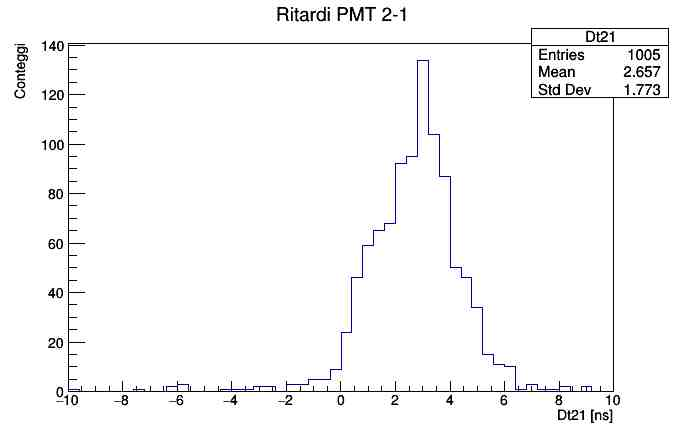
\includegraphics[width=\textwidth]{./immagini/TimeOfFlight/Rit21Fore.jpg}
\caption{}
\label{fig:Dt21Fore}
\end{subfigure}
\hfill
\begin{subfigure}[b]{0.45\textwidth}
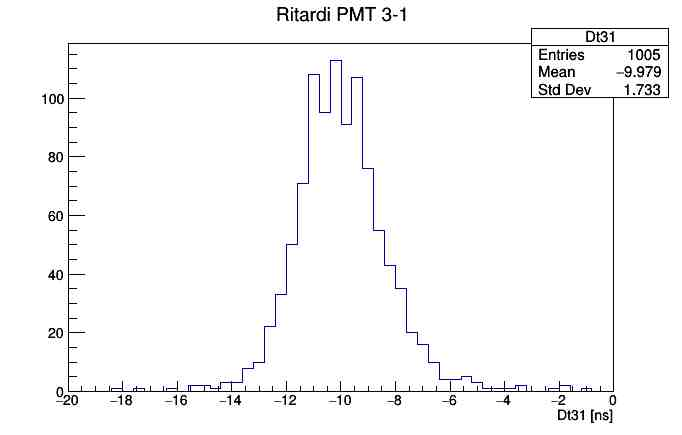
\includegraphics[width=\textwidth]{./immagini/TimeOfFlight/Rit31Fore.jpg}
\caption{}
\label{fig:Dt31Fore}
\end{subfigure}
\hfill
\begin{subfigure}[b]{0.45\textwidth}
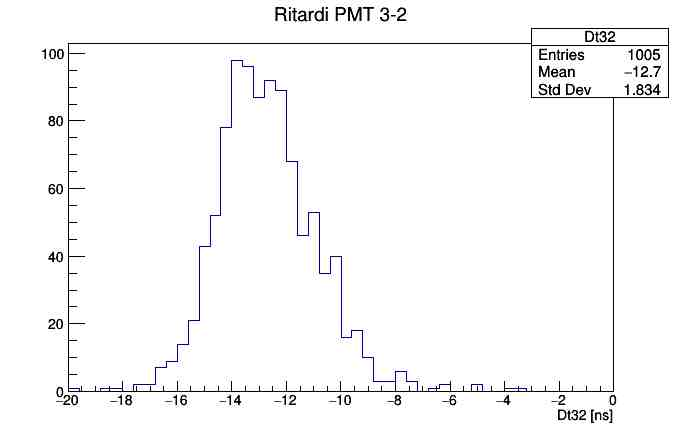
\includegraphics[width=\textwidth]{./immagini/TimeOfFlight/Rit32Fore.jpg}
\caption{}
\label{fig:Dt32Fore}
\end{subfigure}
\end{center}
\caption{Per ognuno degli istogrammi sono stati eseguiti dei fit con una gaussiana, per stimare meglio i ritardi tra i PMT e inseriti i ritardi misurati in tabella\,\ref{tab:RitFore}.}
\label{fig:RitFore}
\end{figure}


\begin{table}[H]
\begin{tabular}{|c|c|c|}
\hline
$R_{21}$ [ns] & $R_{31}$ [ns] & $R_{32}$ [ns] \\
\hline
2,74\:$\pm$\:1,42 & -10,0\:$\pm$\:1,48 & -12,8\:$\pm$\:1.65\\
\hline
\end{tabular}
\caption{}
\label{tab:RitFore}
\end{table}

E dunque la distribuzione di velocità è

\begin{figure}[H]
\centering
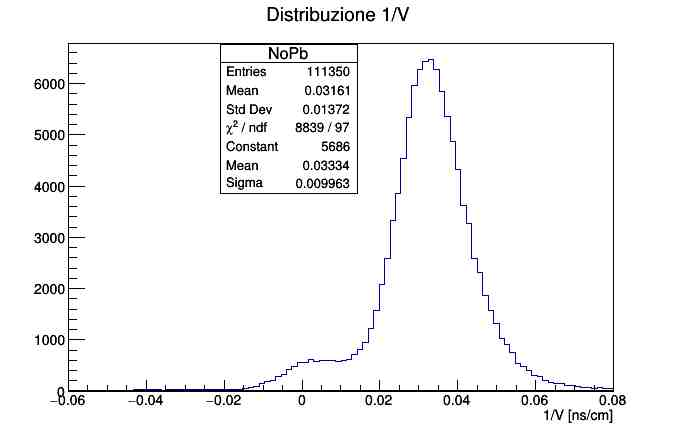
\includegraphics[scale=0.4]{./immagini/TimeOfFlight/Distr1SuV.jpg}
\caption{Si sceglie di utilizzare 1/V per poter mantenere una distribuzione di tipo gaussiana, in quanto V = x/TOF e solo TOF segue una distribuzione gaussiana, mentre x, come si vede dai grafici in sezione\,\ref{sec:Distribuzioni}, non la segue.}
\label{fig:Distr1SuVFore}
\end{figure}

La distribuzione di 1/V in figura\,\ref{fig:Distr1SuVFore} sembra ben centrata su una media di circa 0,0334\:$\pm$\:0.0010\,$\frac{\nano\second}{\centi\metre}$, cioè di 29,9\:$\pm$\:8,9\,$\frac{\centi\metre}{\nano\second}$.\\
La coda della distribuzione di 1/V, che troviamo per velocità molto maggiori della luce, o addirittura negative, non sembra essere dovuta ad un'incorretta stima della posizione di incidenza, ma piuttosto ad errori nella distribuzione di TOF. Infatti, se osserviamo la distribuzione della posizione (x, figura\,\ref{fig:DistrX}), notiamo una buona simmetria rispetto allo 0 e limiti posti a circa $\pm$\:150\,cm dal centro. Ritroviamo, invece, una coda per tempi vicino allo 0, e anche negativi, nella distribuzione di TOF (figura\,\ref{fig:DistrTof}).


\subsection{Prese dati con piombo}
\label{sec:RapportoU-N}
\paragraph{Conti per il piombo}
Osservando la figura\,\ref{fig:Distr1SuVFore}, è stato deciso di provare a tagliare gli eventi con velocità inversa inferiore a 0,05\,$\frac{\nano\second}{\centi\metre}$ (cioè 20\,$\frac{\centi\metre}{\nano\second}$),  perciò

\begin{center}
$v = 20\frac{\centi\metre}{\nano\second} \Rightarrow \beta \simeq \frac{2}{3} \Rightarrow \gamma \simeq 1,3$ \\ $ p=\gamma m \beta \simeq 94.5 \frac{\mega\electronvolt}{\textnormal{c}} $
\end{center}

con m massa del $\mu$\:=\:105.6\,\mega\electronvolt\per\square{c}.\\
Dal sito PDG\footnote{In particolare alla pagina: \url{https:pdg.lbl.gov/2020/AtomicNuclearProperties/MUE/muE_lead_Pb.pdf}; pagina relativa a come si comportano i muoni in funzione della loro energia nel piombo} si vede che muoni con impulso di circa 100\,MeV\per c, per essere teoricamente frenati, necessitano di uno spessore di piombo per unità di densità (CSDA range) di 1,521\,$\frac{\gram}{\centi\square\metre}$. Perciò, sapendo che la densità del piombo vale 11,35\,$\frac{\gram}{\centi\cubic\metre}$, si ricava che servono almeno 1,2-1,4\,cm di piombo per frenare le particelle con $v\:<\:20\,\frac{\centi\metre}{\nano\second}$.\\
Così sono state posizionate tra il PMT-3 e PMT-4 7 lastre di piombo di spessore di 2\,mm ciascuna.

\paragraph{2 metodi}
Data la bassa efficienza del PMT-4 sono stati pensati due metodi, per valutare la quantità di particelle che vengono assorbite dalle lastre di piombo.\\
Il primo metodo è quello di confrontare due istogrammi normalizzati di quadruple senza piombo e quadruple con il piombo\footnote{Per quadruple intendiamo coincidenze tra tutti i 4 PMT: coincidenze C$_{1234}$. Nel nostro caso queste coincidenze sono state ricercate in analisi dati e non triggerate tramite modulo delle coincidenze.}. In questa maniera si eviterebbe il problema di conteggi minori dovuti all'efficienza del PMT-4, in quanto inclusi direttamente nei dati con e senza piombo.\\
Il rapporto che verrà fatto sarà dunque

\begin{equation}
\frac{\textnormal{Quadruple norm. con Pb}}{\textnormal{Quadruple norm. senza Pb}}
\label{equ:RappQuadNorm}
\end{equation}

In alternativa si potrebbe stimare l'efficienza del PMT-4 tramite rapporto di coincidenze quadruple e triple di una presa dati senza piombo lungo la traiettoria di volo delle particelle.
E successivamente si misurerebbero i rapporti tra coincidenze quadruple e triple di prese dati con il piombo, dividendo per l'efficienza precedentemente stimata.\\
Quindi, sapendo che le quadruple lette dall'ADC valgono:
\begin{equation}
N_{\textnormal{Quadruple}} = N_{\textnormal{Eventi positivi}} \cdot \textnormal{Eff} 
\end{equation}
dove per eventi positivi si intendono le particelle che hanno passato il piombo, il numero di eventi che passano il piombo, corretto con l'efficienza, si può trovare tramite rapporto con gli eventi tripli:
\begin{equation}
\frac{\textnormal{N}_{\textnormal{Eventi positivi}}}{N_{\textnormal{Triple}}} = \frac{\textnormal{N}_{\textnormal{Quadruple}}}{\textnormal{Eff}}\cdot\frac{1}{\textnormal{N}_{\textnormal{Triple}}}
\label{equ:VRappMet2}
\end{equation}

Alternativamente possiamo vederlo come un rapporto tra rapporti quadruple/triple tra dati con piombo e senza piombo.
\begin{equation}
\frac{\textnormal{Quadruple con Pb}}{\textnormal{Triple con Pb}} / \frac{\textnormal{Quadruple senza Pb}}{\textnormal{Triple senza Pb}}
\label{equ:RappEff}
\end{equation}

\subsubsection*{Metodo 1: rapporto tra  quadruple normalizzate}
Date due distribuzioni normalizzate (figura\,\ref{fig:DistrQuadNorm}) di eventi che verificano una coincidenza quadrupla C$_{1234}$ con del piombo posizionato tra gli scintillatori 3 e 4, si verifica successivamente il rapporto tra eventi con $v\:>\:20\,\frac{\centi\metre}{\nano\second}$ e quelli non con $v\:<\:20\,\frac{\centi\metre}{\nano\second}$ (vedi figura\,\ref{fig:1SuVRappFore}).

\begin{figure}[H]
\centering
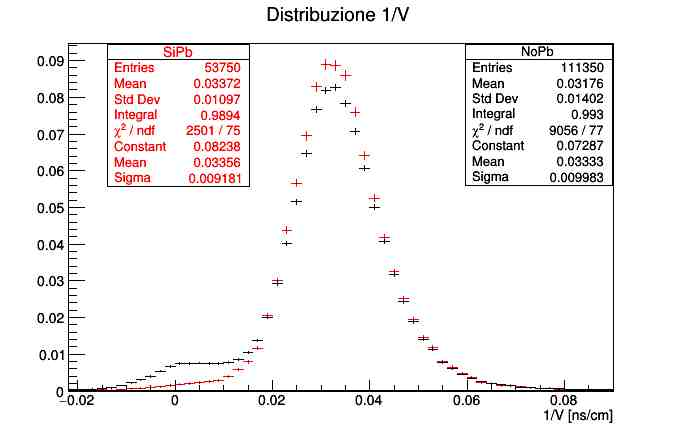
\includegraphics[scale=0.4]{./immagini/TimeOfFlight/Distr1SuVQuadNormFore.jpg}
\caption{In rosso la distribuzione degli eventi con il piombo tra i PMT-3 e PMT-4, in nero quelli senza.}
\label{fig:DistrQuadNorm}
\end{figure}

I risultati dei fit fatti sono riportati in figura\,\ref{fig:DistrQuadNorm}.\\
Adesso si calcola il rapporto tra le distribuzioni di 1/V con e senza piombo di equazione\,\ref{equ:RappQuadNorm}.

\begin{figure}[H]
\begin{center}
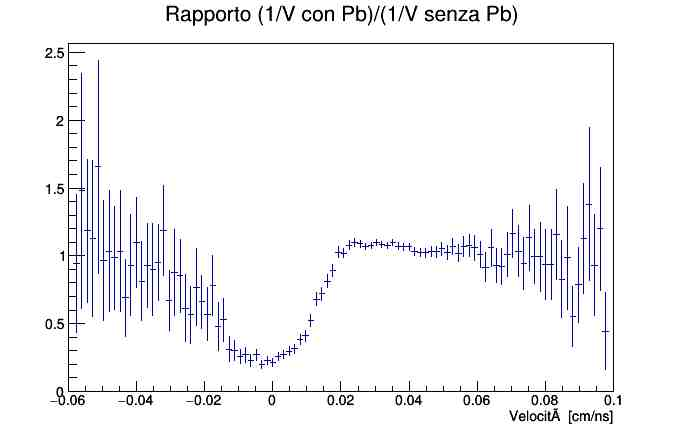
\includegraphics[scale=0.4]{./immagini/TimeOfFlight/Rapp1SuVQuadNorm.jpg}
\end{center}
\caption{Rapporto tra distribuzioni normalizzate.}
\label{fig:1SuVRappFore}
\end{figure}

Per quanto riguarda il rapporto in figura\,\ref{fig:1SuVRappFore} si nota una tendenza a rimanere intorno all'unità con un lieve calare del numero di quadruple rispetto alle triple per 0.05\:>\:1/V\:>\:0.04\,$\frac{\nano\second}{\centi\metre}$, cioè 20\:<\:V\:<\:25\,$\frac{\centi\metre}{\nano\second}$. Si perde, però, questo effetto per 1/V\:>\:0.05\,$\frac{\nano\second}{\centi\metre}$, proprio nella zona desiderata (vedi i 
conti all'inizio di questa sezione\,\ref{sec:RapportoU-N}).\\
Gli integrali calcolati sulle due distribuzioni sono molto vicini tra loro: 0,993 per la presa dati senza piombo e 0,990 per quella con il piombo, ma nel caso della presa dati con il piombo l'assenza della coda a 1/V\:<\:0,015\,$\frac{\nano\second}{\centi\metre}$ ha fatto alzare i valori normalizzati delle velocità interessanti.\\
L'effetto del piombo sembra aver influenzato maggiormente le particelle a velocità molto alte e negative, piuttosto che quelle nella regione interessante per 1/V\:>\:0.05\,$\frac{\nano\second}{\centi\metre}$.

\subsubsection*{Metodo 2, misura dell'efficienza}
\label{sec:Met2}
Si prova questo secondo metodo per poter utilizzare lo stesso set di eventi, così da evitare distribuzioni di eventi molto diverse tra loro, oppure di normalizzazioni differenti per effetti al momento sconosciuti dovuti allo scintillatore 4.

\paragraph{Efficienza PMT-4}
Cominciamo con l'efficienza del PMT-4, ovvero il rapporto tra eventi tripli (C$_{123}$) e quadrupli (C$_{1234}$) senza piombo tra gli scintillatori 3 e 4.

\begin{figure}[H]
\centering
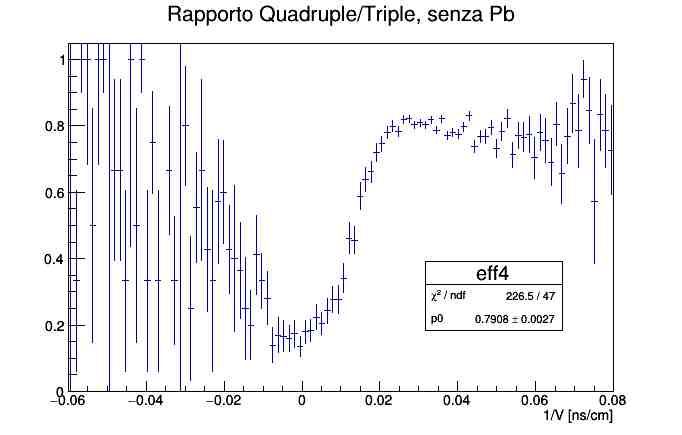
\includegraphics[scale=0.4]{./immagini/TimeOfFlight/1SuVEffFore.jpg}
\caption{Rapporto $\frac{\textnormal{Quadruple}}{\textnormal{Triple}}$ senza piombo tra i PMT. Gli errori sono stati valutati come per le calibrazioni (vedi sezione "Distribuzione Binomiale"\,\ref{sec:DistrBino}).}
\label{fig:1SuVEffFore}
\end{figure}

In figura\,\ref{fig:1SuVEffFore} è riportato il valore di un fit di una retta costante sui valori di 1/V\:>\:0.02\,$\frac{\nano\second}{\centi\metre}$ (50\,$\frac{\centi\metre}{\nano\second}$), corrispondente ad una stima dell'efficienza del PMT-4.\\
Procediamo, dunque, con la stima delle particelle fermate dal piombo (equazione\,\ref{equ:RappEff}).

\begin{figure}[H]
\centering
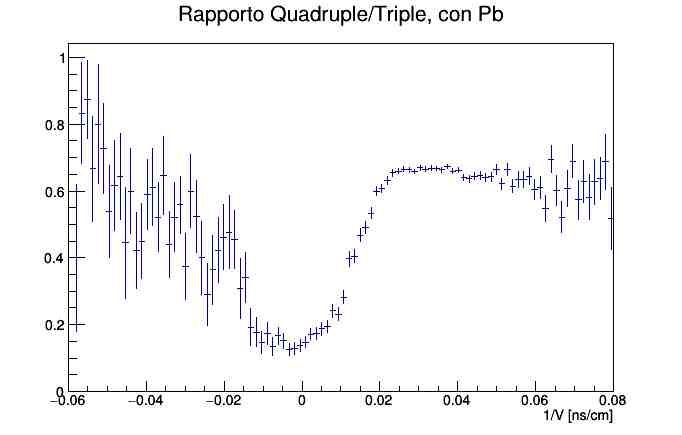
\includegraphics[scale=0.4]{./immagini/TimeOfFlight/1SuVRappPiomboFore.jpg}
\caption{}
\label{fig:1SuVRappPbFore}
\end{figure}

E successivamente si corregge la distribuzione in figura\,\ref{fig:1SuVRappPbFore} come da equazione\,\ref{equ:VRappMet2}.

\begin{figure}[H]
\centering
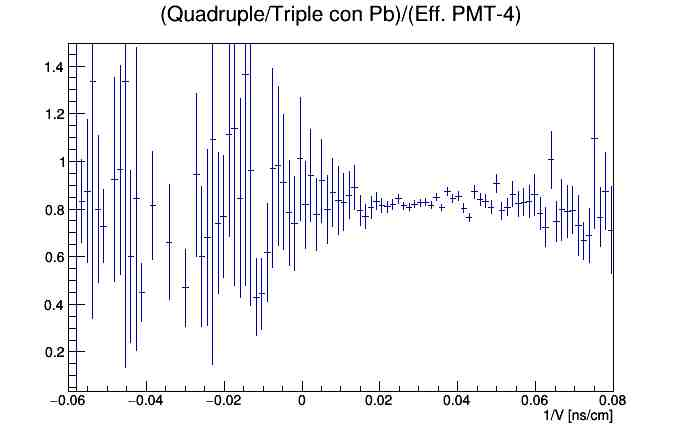
\includegraphics[scale=0.4]{./immagini/TimeOfFlight/1SuVRappPbEffFore.jpg}
\caption{}
\label{fig:1SuVRappPbEffFore}
\end{figure}

Osservando le figure\,\ref{fig:1SuVEffFore} e \ref{fig:1SuVRappPbFore}, notiamo che per 1/V\:>0.03\,$\frac{\nano\second}{\centi\metre}$ il rapporto tende a diminuire, ma molto lievemente.\\
Come prima cosa, se osserviamo la regione 0.02\,$\frac{\nano\second}{\centi\metre}$\:<\:1/V\:<\:0.05\,$\frac{\nano\second}{\centi\metre}$, in entrambe le figure notiamo che nel caso con il piombo il rapporto si trova ad un valore più basso. Ciò porta a pensare che il piombo abbia effettivamente frenato delle particelle.\\
Quello però che non piace è che il piombo sembra aver frenato equamente particelle a tutte le velocità, poiché, osservando la figura\,\ref{fig:1SuVRappPbEffFore} i valori del rapporto tendono a rimanere stabili a tutti i valori di 1/V, come se l'effetto dell'efficienza del PMT-4 fosse molto più influente rispetto a quello del piombo.



\newpage
\section{Attenuazione segnale luminoso}
\label{sec:Atte}
L'efficienza di rivelazione delle particelle è data anche dalla probabilità del segnale luminoso di raggiungere gli estremi dello scintillatore.\\
L'energia persa segue teoricamente un andamento esponenziale del tipo
\begin{equation}
L(x) = L_0e^{-\frac{x}{l}}
\label{equ:AttLuce}
\end{equation}
dove L$_0$ è la luminosità iniziale del segnale e l la lunghezza di attenuazione\footnote{Si definisce lunghezza di attenuazione la lunghezza per la quale la luminosità si riduce di un fattore $\frac{1}{e}$.}.

\subsection{Dipendenza dalla posizione}
\label{sec:AttPos}
Per questa misura sono stati presi alcuni ritardi tra PMT-1 e PMT-2, se ne è ricostruita la posizione di incidenza nella barra, usando l'equazione\,\ref{equ:PosX}, e si è eseguito uno scatterplot delle cariche viste da un PMT, in questo caso il PMT-1.

\begin{figure}[H]
\begin{subfigure}[b]{0.45\textwidth}
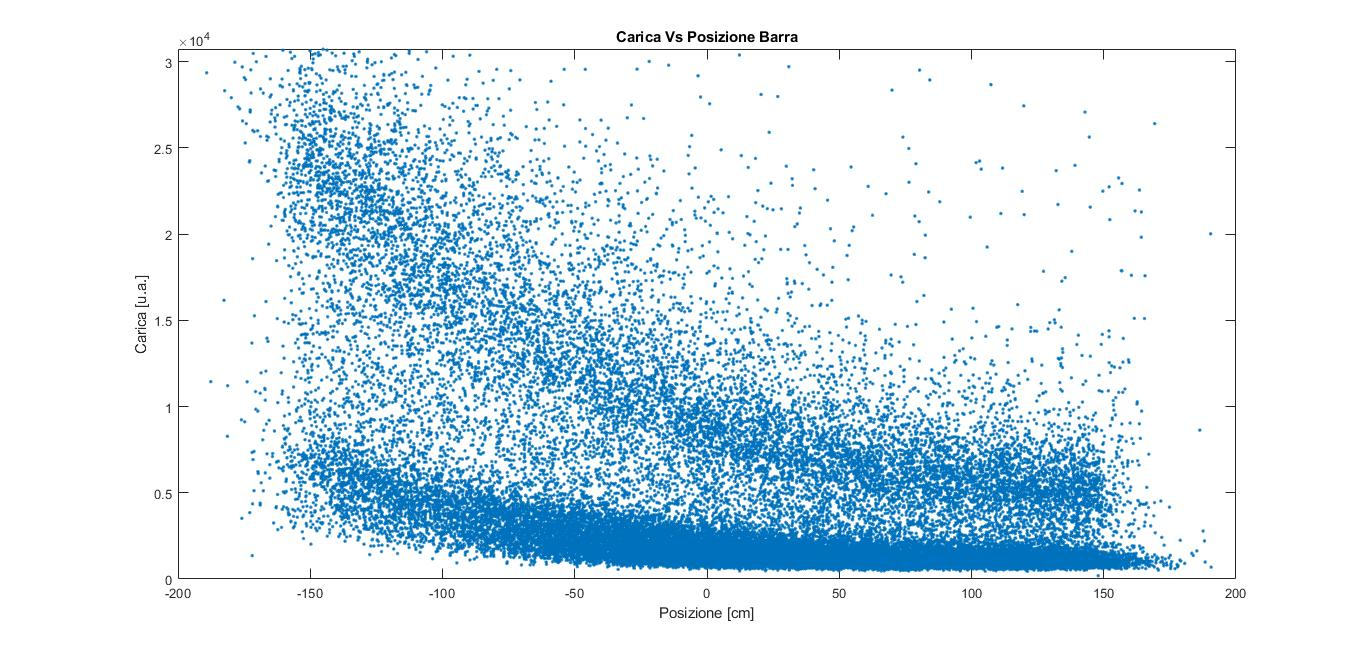
\includegraphics[width=\textwidth]{./immagini/TimeOfFlight/AttenuazioneDoppia.jpg}
\caption{}
\label{fig:AttenuazioneDoppia}
\end{subfigure}
\hfill
\begin{subfigure}[b]{0.45\textwidth}
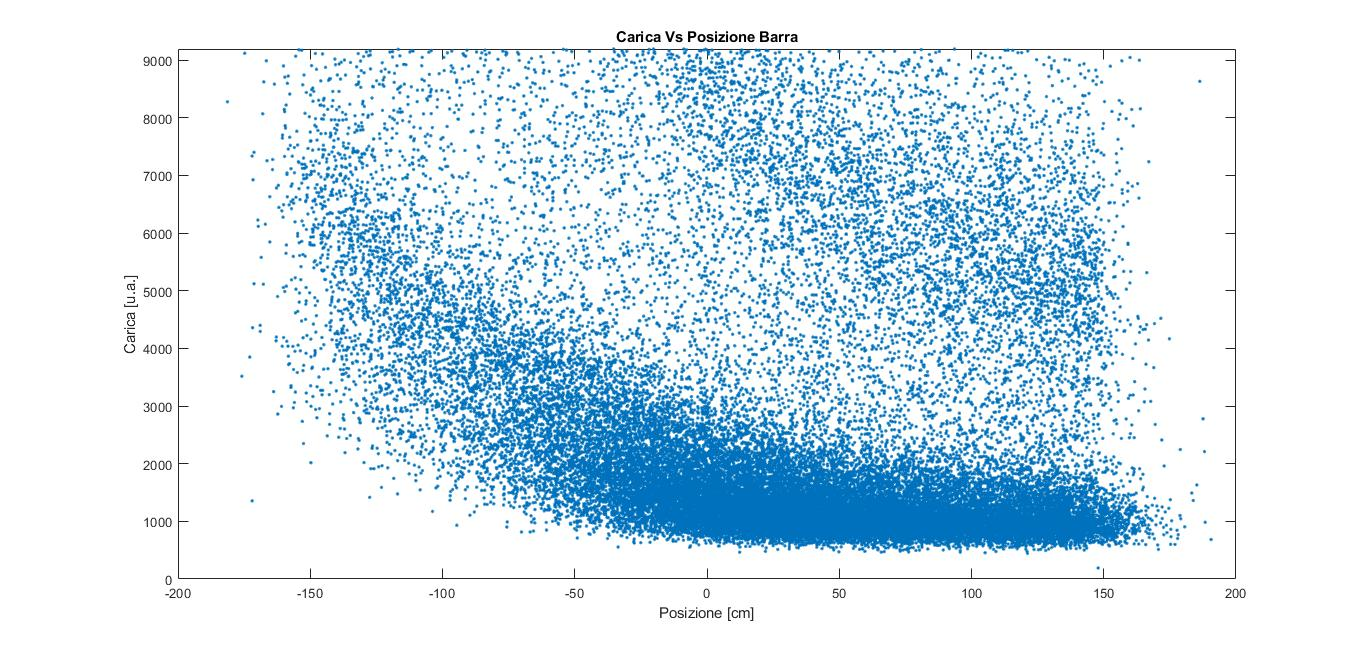
\includegraphics[width=\textwidth]{./immagini/TimeOfFlight/AttenuazioneDoppiaZoom.jpg}
\caption{Zoom sui dati inferiori in figura\ref{fig:AttenuazioneDoppia}}
\label{fig:AttenuazioneDoppiaZoom}
\end{subfigure}
\hfill
\begin{subfigure}[b]{0.45\textwidth}
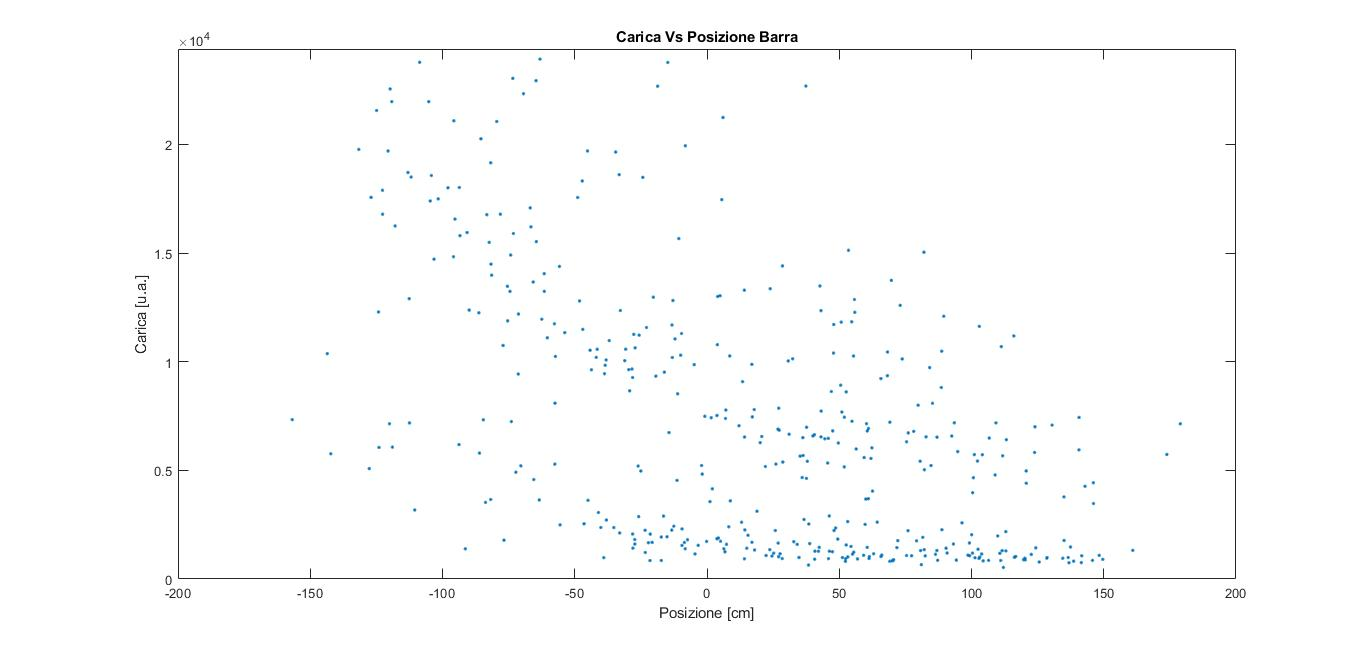
\includegraphics[width=\textwidth]{./immagini/TimeOfFlight/AttenuazioneTripla.jpg}
\caption{Coincidenze triple ricavate dai dati della figura\,\ref{fig:AttenuazioneDoppia}}
\label{fig:AttenuazioneTripla}
\end{subfigure}
\caption{}
\end{figure}

Dalla figura\,\ref{fig:AttenuazioneDoppia} si nota un andamento di tipo esponenziale comune a due fasce di eventi (\ref{fig:AttenuazioneDoppiaZoom}).\\
Tutti quei segnali nella fascia più bassa, sappiamo non essere dipendenti dalla luce, perché i conteggi in singola con luce accesa o spenta non variano.\\
\'E stata fatta una prova per vedere quali fossero segnali di rumore, trovando le coincidenze triple con gli stessi dati.\\
Nonostante questo riconoscimento delle triple dei dati in figura\,\ref{fig:AttenuazioneDoppia} notiamo dallo scaterplot\,\ref{fig:AttenuazioneTripla} nuovamente la presenza di segnali con energie inferiori.\\
Come si vede maggiormente dalla figura\,\ref{fig:AttenuazioneTriplaFitta} questi dati sono effettivamente delle particelle passanti per il sistema, poiché ottenuti tramite coincidenze triple tra i PMT(1-2-3).

\begin{figure}[H]
\flushleft
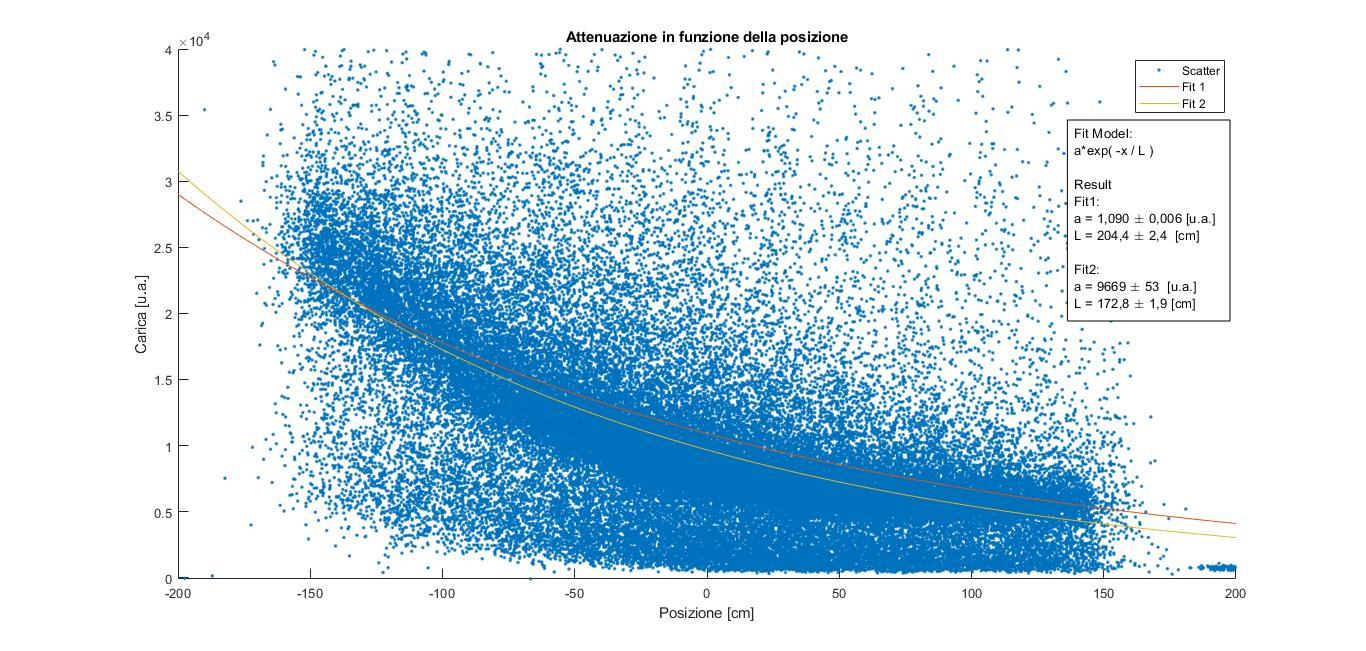
\includegraphics[width=0.53\textwidth]{./immagini/TimeOfFlight/AttenuazioneMatlab.jpg}
\caption{Dati riferiti alle triple prese per la distribuzione di V con il piombo}
\label{fig:AttenuazioneTriplaFitta}
\end{figure}

Per valutare l'effettivo andamento dei dati sono stati provati due fit con il modello di equazione\,\ref{equ:AttLuce} dove L$_0 = a$.\\
Nel caso del Fit-1 sono stati tagliati i dati a bassa intensità; nel secondo, Fit-2, sono stati considerati anche quelli.\\
I risultati in figura sembrano avvicinarsi alla lunghezza di attenuazione, di 210\,cm, indicata nel datasheet della barra scintillante.\\
Inoltre, se facciamo un rapporto tra la misura di L$_0$ e la lunghezza di attenuazione del datasheet, e facciamo la stessa cosa con la velocità della luce nella barra scintillante, troviamo che:

\begin{center}
$\frac{v_{luce}\:Teorica}{v_{luce}\:Misurata} = 1,24 \sim \frac{L_0\:Teorica}{L_0\:Misurata} = 1,22$
\end{center}

Questo porterebbe a pensare che l'effetto dovuto alla non linearità del percorso dei fotoni all'interno della barra sia equo per entrambe le misure\footnote{Dato che per la misura di v non si sono fate distinzioni tra cariche di un certo valore o meno è stato ritenuto fare quest'ultima considerazione utilizzando i risultati del fit dove venivano valutati tutti i segnali, Fit-2}.

\subsection{Dipendenza dall'angolo}
\label{sec:Angolo}
Per valutare la carica dei segnali luminosi rivelati dai PMT, si deve considerare la distanza percorsa dalla particella nella barra; la distanza ha una dipendenza dall'angolo con il quale la particella incide sulla barra. Infatti, a seconda dell'angolo di incidenza, la particella compierà un cammino più o meno lungo nella barra, e rilascerà di conseguenza un maggiore energia per un percorso più lungo effettuato.\\
Per visualizzare quale sia la dipendenza dall'angolo di incidenza della particella sulla barra, è stato necessario eliminare prima la dipendenza dalla posizione. Per fare ciò è stato pensato il seguente metodo:\\
sapendo che la carica vista dal PMT-1 segue la legge
\begin{equation}
C_1(x) = C_1 f(\theta)e^{(-\frac{\frac{L}{2}+x}{l})}
\end{equation}
e per il PMT-2
\begin{equation}
C_2(x) = C_2f(\theta)e^{(-\frac{\frac{L}{2}-x}{l})}
\end{equation}
dove $f(\theta)$ è una dipendenza dall'angolo in questione, facendo il prodotto tra le due cariche si ricava
\begin{equation}
C_1(x)C_2(x) = f(\theta)^2 C_1C_2 e^{-\frac{L}{l}}
\end{equation}

dove però anche $C_1$ e $C_2$ dipendono da $\theta$.\\
Per tanto il prodotto tra gli integrali del segnale diventa una funzione solo di $\theta$.\\
Data la simmetria del nostro apparato sperimentale, è possibile trasformare la dipendenza da $\theta$ in quella della posizione tramite una semplice trasformazione
\begin{equation}
cos(\theta) = \frac{h}{d}
\label{equ:XtoTheta}
\end{equation}
dove h è l'altezza della barra scintillante rispetto allo scintillatore 3.

\begin{figure}[H]
\centering
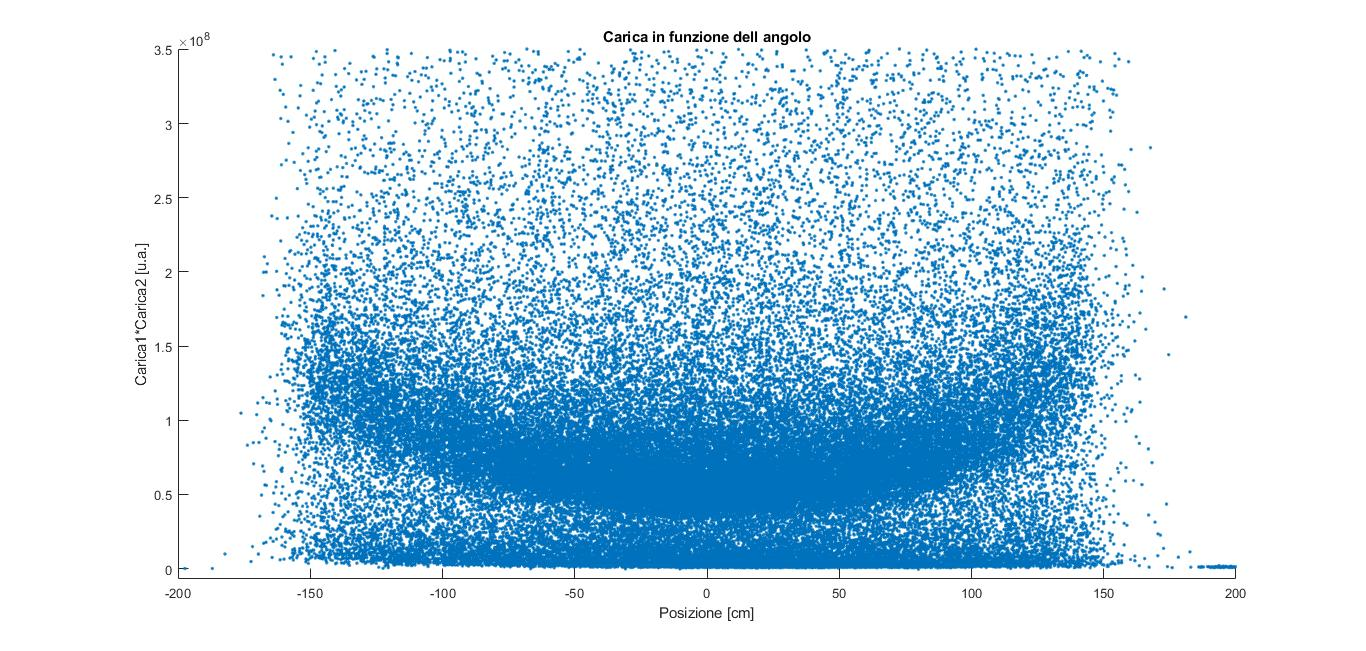
\includegraphics[width=0.5\textwidth]{./immagini/TimeOfFlight/DipendenzaAngolo.jpg}
\caption{Limiti per l'angolo cos($\theta$)\.<\:|0,76|, quindi $\theta$\:<\:|40|. Vedi anche figura \ref{fig:DistrTheta}}
\label{fig:DipendenzaAngolo}
\end{figure}

Dai dati usati in figura\,\ref{fig:DipendenzaAngolo} è stato inoltre possibile valutare quanti fossero gli eventi a cariche maggiori rispetto a quelli minori, tramite la visualizzazione con un istogramma simile a quello di figura\,\ref{fig:RappSiMe}.\\
\'E stato stimato circa l' 80$\%$ di particelle con energia rilasciata nella barra più alta.
\begin{center}
Cariche Alte/Tot Eventi $\simeq$\:61810/76452\:=\:80$\%$ 
\end{center}


\newpage
\section{Altre distribuzioni}
\label{sec:Distribuzioni}
\begin{figure}[H]
\begin{subfigure}[b]{0.4\textwidth}
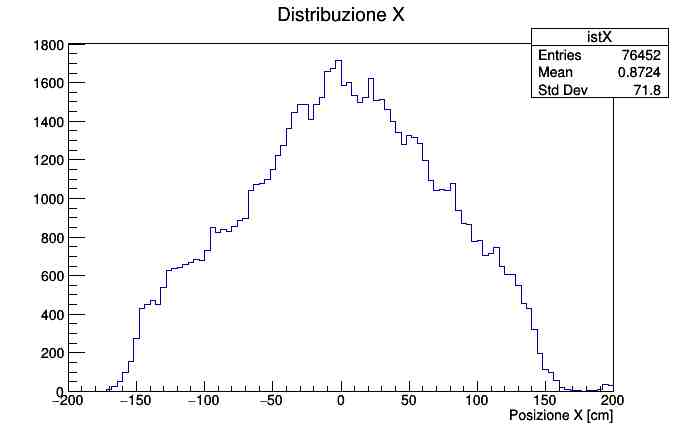
\includegraphics[width=\textwidth]{./immagini/TimeOfFlight/DistrX.jpg}
\caption{Ricavata con l'equazione \ref{equ:PosX}}
\label{fig:DistrX}
\end{subfigure}
\hfill
\begin{subfigure}[b]{0.4\textwidth}
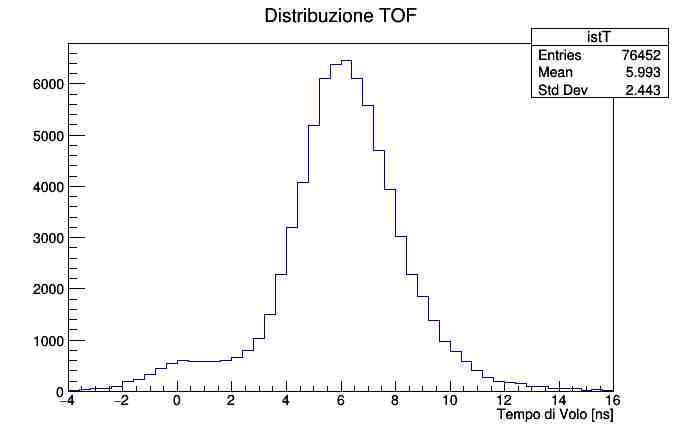
\includegraphics[width=\textwidth]{./immagini/TimeOfFlight/DistrTOF.jpg}
\caption{Tempo di volo misurato con la media tra TOF$_1$ e TOF$_2$ come in equazione\,\ref{equ:TOF}}
\label{fig:DistrTof}
\end{subfigure}
\caption{}
\end{figure}

\begin{figure}[H]
\begin{subfigure}[b]{0.4\textwidth}
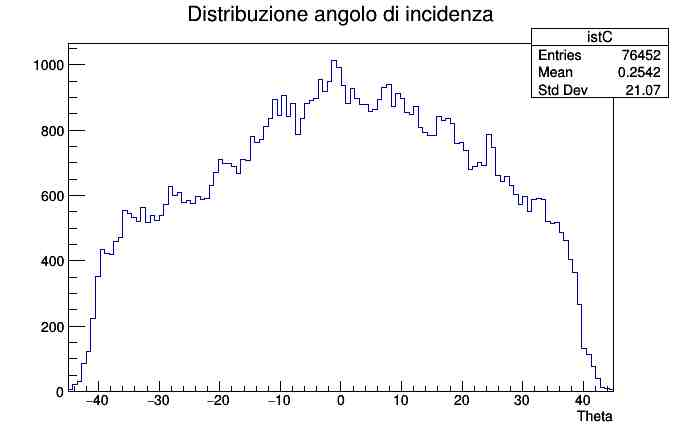
\includegraphics[width=\textwidth]{./immagini/TimeOfFlight/DistrTheta.jpg}
\caption{$\theta = arccos(\frac{h}{d})$}
\label{fig:DistrTheta}
\end{subfigure}
\hfill
\begin{subfigure}[b]{0.4\textwidth}
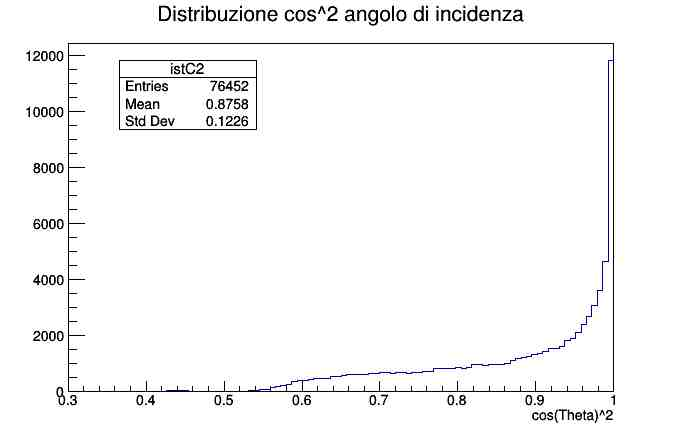
\includegraphics[width=\textwidth]{./immagini/TimeOfFlight/DistrCos2.jpg}
\caption{}
\label{fig:DistrCos2}
\end{subfigure}
\caption{}
\end{figure}










\newpage
\appendix
\section{Problemi affrontati}
\label{sec:AProblemiADC}
La procedura seguita per migliorare le nostre misure parte dal riconoscimento dell'evento presumibilmente ricostruito male, o riportante come risultato una velocità molto lontana dalle aspettative, visualizzandolo successivamente con un semplice plot dei dati acquisiti con l'ADC.\\
Alcuni errori sono stati commessi nei codici di analisi dati, altri invece sono stati causati dalle caratteristiche dell'ADC.\\
Di seguito sono riportati alcune correzioni e errori commessi nell'ordine in cui sono stati trovati.\\
Durante la descrizione dei problemi saranno indicate alcune delle funzioni scritte e utilizzate per l'analisi dati\footnote{In appendice \ref{sec:ARep} trovate il link al repositorio online.}.

\subsection{"Coincidenze casuali", ADC Record Lenght}
\label{sec:ARecLenght}
Il primo problema è legato alla lunghezza del record di dati che l'ADC restituisce, ogni qual volta scatti il trigger, impostato generalmente su una tripla C$_{123}$.\\
Una delle cause che faceva risultare una particella molto lenta consisteva nella presenza di un secondo evento\footnote{Per secondo evento intendiamo dei segnali rivelati da un solo PMT o da più insieme, in pratica osservavamo più doppie o più segnali singoli su un solo PMT nello stesso record di dati.} nello stesso record di dati.\\
Questa "coincidenza casuale" faceva sì che il codice di analisi dati riportasse come $\Delta t$ un intervallo di tempo tra due impulsi relativi a due eventi diversi e non allo stesso.\\
Infatti, facendo un semplice conto, la possibilità che due eventi vengano registrati nello stesso record di dati non è così bassa.\\
Partiamo dal fatto che un record è lungo 1030 campioni, cioè, sapendo che l'ADC campiona con una frequenza di 250\,MHz, ogni campione dista temporalmente dai vicini 4\,ns, e quindi in totale si ha una finestra in tempi di 4,12\,\micro\second. Calcolando la possibilità che due PMT possano rivelare due eventi distinti entro la finestra temporale di 4,12\,\micro\second, si ottiene:

\begin{equation}
f_{cas} = f_1 \cdot f_2 \cdot \tau = 10^2 \textnormal{ cps} \cdot 10^2\textnormal{ cps} \cdot 10^{-6} \space \mu\textnormal{s} = 10^{-2} \textnormal{ cps}
\end{equation}

cioè, 1 ogni 100 eventi potrebbe presentare due eventi su un unico record di dati.\\
Per rimediare a questo problema, è stato pensato di scrivere una funzione che funzionasse come un trigger sui dati da analizzare.\\
Questo ha inoltre permesso di trovare eventuali coincidenze tra segnali provenienti da PMT che non erano messi in coincidenza tramite il modulo NIM apposito; tutte le quadruple, per esempio, sono state ricercate in analisi dati e non tramite trigger esterno.\\
Per riuscire a scrivere questo trigger, è stato necessario discriminare i minimi relativi dei record di dati e perciò riconoscere quale minimo fosse di rumore, e quale del segnale stesso.

\subsubsection{Analisi dati, ricerca dei minimi}
\label{sec:AThreshold}
Entriamo più in dettaglio su questa ricerca dei minimi. Dobbiamo partire dalla descrizione di una funzione che sistemi i dati ricevuti dall'ADC.
\paragraph{Function: GestioneOff}
Ogni evento ricostruito dall'ADC si presentava rialzato dallo 0 di un offset di circa 14700\,ua. Per sistemare questo offset, è stato necessario settare delle soglie molto intuitive, osservando qualche evento casualmente. Sono stati selezionati tutti i dati con carica compresa tra le due soglie e sono stati ricavati un offset ("off") come media dei valori di rumore, e una "Sigma", deviazione standard di questi valori.\\
L'offset è stato utilizzato per spostare i dati sullo zero, mentre la sigma è stata utilizzata per ricercare i minimi relativi nel record di dati proveniente dall'ADC, in particolare è stata utilizzata nella funzione descritta di seguito.
\paragraph{Function: ThrsDet}
Questa funzione legge i dati provenienti dai singoli PMT, ricerca il minimo assoluto di un singolo evento per volta e utilizza il valore di sigma calcolata per lo stesso evento e ne restituisce un array con tutti i rapporti $\frac{\textnormal{Sigma}}{\textnormal{Absolute min}}$ del record di dati del PMT.

\begin{figure}
\centering
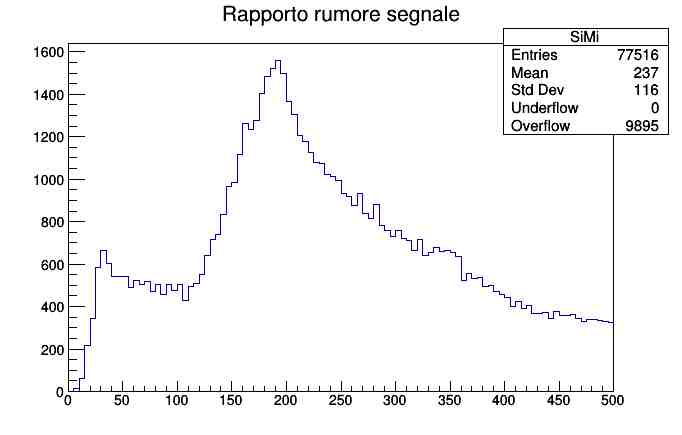
\includegraphics[scale=0.4]{./immagini/TimeOfFlight/RappRumSeg.jpg}
\caption{La figura riporta l'istogramma dei rapporti (sigma rumore)/(minimo ass. segnale) di una serie di eventi rivelati dal PMT-1.}
\label{fig:RappSiMe}
\end{figure}

Osservando dunque grafici come quelli di figura\,\ref{fig:RappSiMe}, per ogni evento si è deciso di tagliare meno campioni possibile, ricercando nei record di dati i minimi relativi che fossero minori più di circa 15 volte la devstd della misura sul rumore dell'evento stesso.
\paragraph{Function: TripleRecognize}
Infine, per decidere quale minimo relativo fosse quello della tripla effettivamente triggerante, si è scelto di tenere i minimi relativi più bassi di ogni PMT, che non distassero tra di loro più di una finestra oltre i 13 campioni, cioè 52\,ns.\\
Utilizzando queste funzioni, è stato inoltre possibile eliminare alcuni dei segnali come quelli in figura\,\ref{fig:FalsaTripla}.

\begin{figure}
\centering
\title{Falsa tripla}
\begin{center}
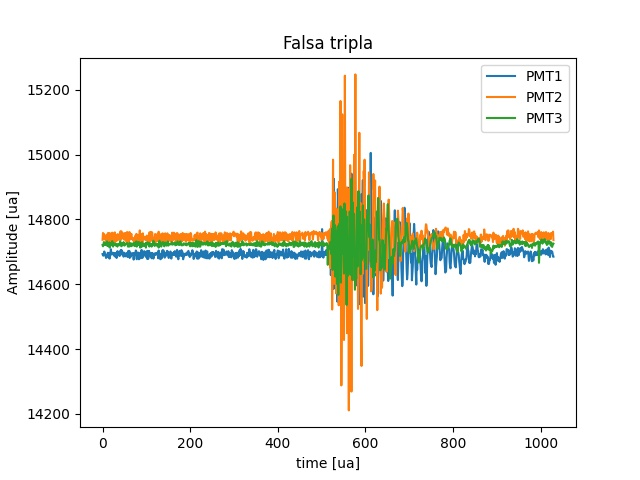
\includegraphics[scale=0.4]{./immagini/TimeOfFlight/FalsaTripla.jpg}
\caption{Sono stati trovati con percentuali sotto l'1$\%$ segnali di questo tipo in tutte le prese dati}
\label{fig:FalsaTripla}
\end{center}
\end{figure}

\subsection{Segnali mal riprodotti, "ADC Sample Rate"}
\label{sec:ATentativi}
L'altra limitazione che è stata riscontrata è quella dovuta al rate di campionamento dell'ADC.\\
L'ADC N6725S campiona con una frequenza di 250\,MHz, cioè un campione ogni 4\,ns e, sapendo che i segnali sono in media lunghi dai 15\,ns ai 20\,ns e sono di tipo impulsivo, la ricostruzione di questi, in particolare del picco, da parte dello strumento può non essere ottimale.\\
Di conseguenza la misura del time-stamp può non essere precisa o addirittura sbagliata.

\subsubsection{Time-stamp}
Di solito con time-stamp di un segnale impulsivo si considera l'istante in cui esso raggiunge il 50$\%$ in ampiezza del valore minimo del segnale. Inoltre, si considerano inizio e fine del segnale, i momenti in cui  questi passano rispettivamente le soglie del 10$\%$ e del 90$\%$.\\
Queste due operazioni però non sono state possibili, in quanto determinati segnali impulsivi raggiungevano il minimo, partendo da sotto il 10$\%$, con un solo dato dell'ADC, cioè con un tempo inferiore a 4\,ns. Questo valeva sia per segnali poco energetici che per alcuni molto energetici, che non venivano di conseguenza riconosciuti dalle funzioni.\\
Per misurare il time-stamp sono state fatte diverse prove; se ne mostrano le differenze tramite gli istogrammi dei ritardi tra le trasmissioni dei PMT-2 e PMT-1, la distribuzione di V\footnote{il calcolo di time-stamp ha una propria funzione chiamata "TimeStampMeas". Mentre le funzioni che determinano l'inizio e la fine di un segnale utilizzando la sigma si chiamano findstart e findstop} e i risultati dei fit con una gaussiana su tutte le distribuzioni dei ritardi tra i PMT.

\paragraph{Media della discesa del segnale}
Per questa prima prova si considera come time-stamp la media dei punti che formano la discesa del segnale, considerando anche i campioni sotto il 10$\%$ e sopra il 90$\%$.

\begin{figure}[H]
     \centering
     \title{Media della discesa del segnale}
     \begin{center}
     \begin{subfigure}[b]{0.4\textwidth}
         \centering
         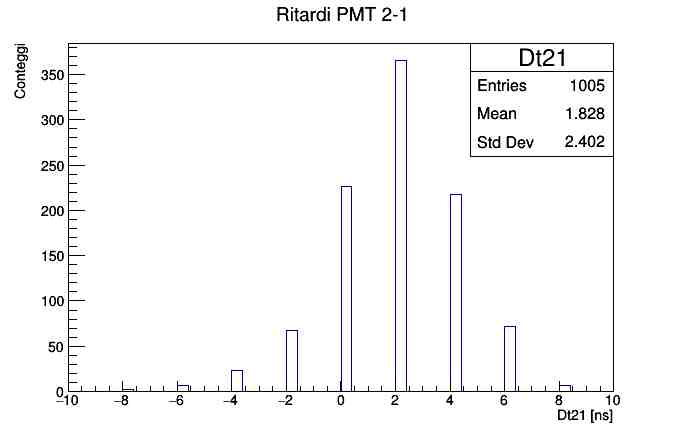
\includegraphics[width=\textwidth]{./immagini/TimeOfFlight/Rit21MidNegSlo.jpg}
         \caption{50 bin nella finestra (-10$\rightarrow$10)\,ns}
         \label{fig:Dt21MidNegSlo}
     \end{subfigure}
     \hfill
     \begin{subfigure}[b]{0.4\textwidth}
         \centering
         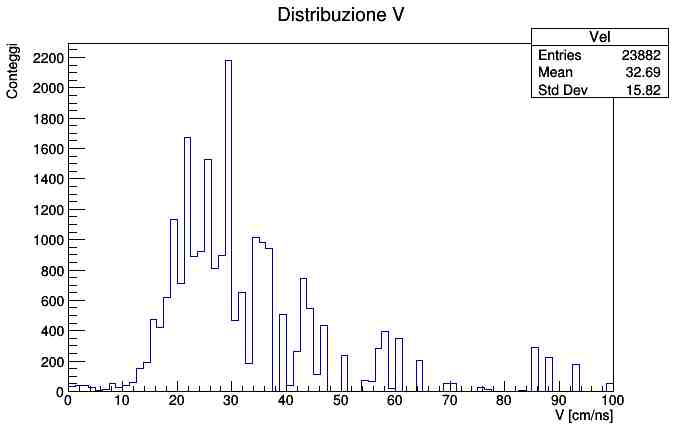
\includegraphics[width=\textwidth]{./immagini/TimeOfFlight/VMidNegSlo.jpg}
         \caption{}
         \label{fig:VMidNegSlo}
     \end{subfigure}
     \end{center}
     \caption{}        
     \label{fig:MidNegSlo}
\end{figure}

\begin{table}[H]
\begin{tabular}{c|c|c}
$R_{21}$ [ns] & $R_{31}$ [ns] & $R_{32}$ [ns] \\
\hfill
2,13 $\pm$ 2,25 & -9.07 $\pm$ 2,19 & -11,0 $\pm$ 2,53
\hfill
\end{tabular}
\caption{}
\label{tab:RitMidNegSlo}
\end{table}
I risultati sono troppo discreti, la riproduzione di V troppo larga e con picchi troppo marcati.


\paragraph{Baricentro discesa del segnale}
Per evitare la discretizzazione ci è stato suggerito di provare a fare la stima del baricentro del segnale, per trovare dunque un tempo nel quale fosse passato il segnale stesso.\\
Come primo tentativo si è provato a calcolare il baricentro della sola parte di discesa del segnale, cioè dal suo punto di partenza al suo punto di minimo.

\begin{figure}[H]
     \centering
     \title{Baricentro della discesa del segnale}
     \begin{center}
     \begin{subfigure}[b]{0.4\textwidth}
         \centering
         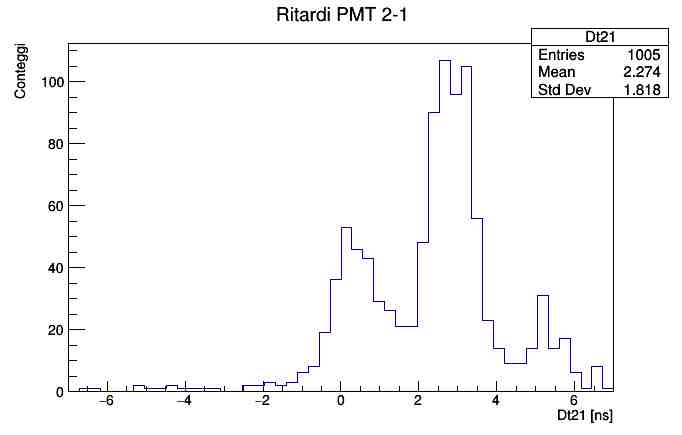
\includegraphics[width=\textwidth]{./immagini/TimeOfFlight/Rit21IntNegSlo.jpg}
         \caption{}
         \label{fig:Dt21IntNegSlo}
     \end{subfigure}
     \hfill
     \begin{subfigure}[b]{0.4\textwidth}
         \centering
         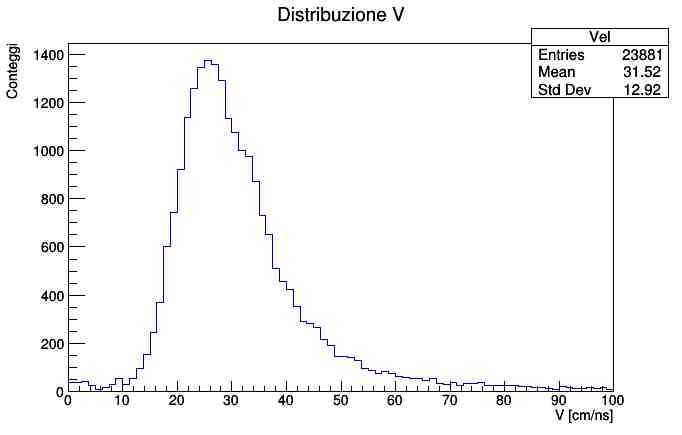
\includegraphics[width=\textwidth]{./immagini/TimeOfFlight/VIntNegSlo.jpg}
         \caption{}
         \label{fig:VIntNegSlo}
     \end{subfigure}
     \end{center}
     \caption{}        
     \label{fig:IntNegSlo}
\end{figure}

\begin{table}[H]
\begin{tabular}{c|c|c}
$R_{21}$ [ns] & $R_{31}$ [ns] & $R_{32}$ [ns] \\
\hfill
2,23 $\pm$ 1,72 & -9.47 $\pm$ 1.81 & -11,7 $\pm$ 2,06
\hfill
\end{tabular}
\caption{}
\label{tab:RitIntNegSlo}
\end{table}

Non si nota più la discretizzazione dei risultati del paragrafo precedente, ma la misura del ritardo (figura\,\ref{fig:Dt21IntNegSlo}) non assomiglia ad una gaussiana come da attese.\\
Anche la distribuzione di V è molto migliorata, ma con media e devstd ancora alte.

\paragraph{Baricentro del segnale}
Per questa prova prendiamo il baricentro del segnale, facendone la media dal suo primo campione discriminato, grazie alla funzione findstart, fino al suo ultimo, determinato dalla funzione findstop.

\begin{figure}[H]
     \centering
     \title{Baricentro del segnale}
     \begin{center}
     \begin{subfigure}[b]{0.4\textwidth}
         \centering
         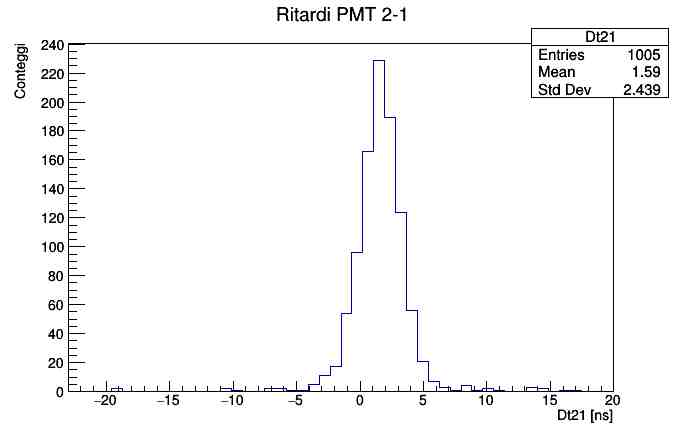
\includegraphics[width=\textwidth]{./immagini/TimeOfFlight/Rit21IntSinTot.jpg}
         \caption{}
         \label{fig:Dt21IntSigTot}
     \end{subfigure}
     \hfill
     \begin{subfigure}[b]{0.4\textwidth}
         \centering
         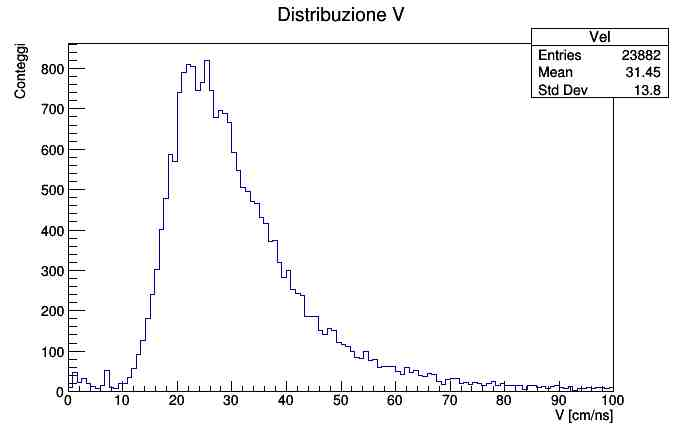
\includegraphics[width=\textwidth]{./immagini/TimeOfFlight/VIntSigTot.jpg}
         \caption{}
         \label{fig:VIntSinTot}
     \end{subfigure}
     \end{center}
     \caption{}        
     \label{fig:IntSinTot}
\end{figure}

\begin{table}[H]
\begin{tabular}{c|c|c}
$R_{21}$ [ns] & $R_{31}$ [ns] & $R_{32}$ [ns] \\
\hfill
1,58 $\pm$ 1,56 & -13,3 $\pm$ 2,07 & -14,9 $\pm$ 2,13
\hfill
\end{tabular}
\caption{}
\label{tab:RitIntSigTot}
\end{table}

La distribuzione del ritardo in figura\,\ref{fig:Dt21IntSigTot}, non presenta più doppi picchi, seppur rimanga piuttosto larga proprio come nel caso della distribuzione di V (\ref{fig:VIntSinTot}).

\paragraph{Baricentro segnale, largo}
Per questa prova si è pensato di allargare la finestra con la quale si esegue la media, per il calcolo del baricentro, così da essere sicuri di prendere tutto il segnale.\\
Eventuali campioni vicini allo zero non influiscono molto sul conto.

\begin{figure}[H]
     \centering
     \title{Baricentro del segnale con qualche dato in più}
     \begin{center}
     \begin{subfigure}[b]{0.4\textwidth}
         \centering
         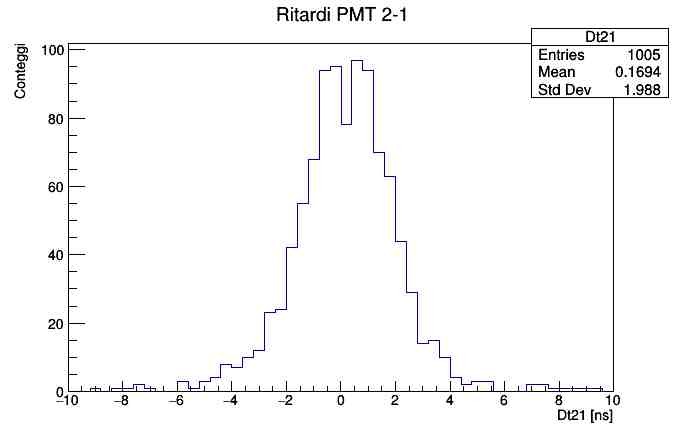
\includegraphics[width=\textwidth]{./immagini/TimeOfFlight/Rit21Largo.jpg}
         \caption{}
         \label{fig:Dt21Largo}
     \end{subfigure}
     \hfill
     \begin{subfigure}[b]{0.4\textwidth}
         \centering
         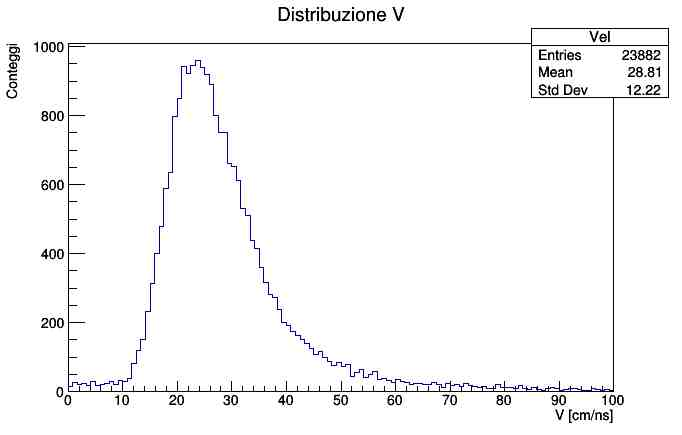
\includegraphics[width=\textwidth]{./immagini/TimeOfFlight/VLargo.jpg}
         \caption{}
         \label{fig:VLargo}
     \end{subfigure}
     \end{center}
     \caption{Per fare queste misure i time stamp sono stati valutati prendendo il baricentro di tutto il segnale, considerando come inizio e fine del segnale 5 unità di tempo in più del tempo di start e 5 meno dello stop, cioè 20\,ns sia a destra che a sinistra del segnale.}        
     \label{fig:Largo}
\end{figure}

\begin{table}[H]
\begin{tabular}{c|c|c}
$R_{21}$ [ns] & $R_{31}$ [ns] & $R_{32}$ [ns] \\
\hfill
0,19 $\pm$ 1,64 & -14,8 $\pm$ 2,17 & -14,9 $\pm$ 2,31
\hfill
\end{tabular}
\caption{}
\label{tab:RitLargo}
\end{table}

Tra i tentativi effettuati questo è l'unico caso per cui si ha un ritardo $R_{21}$, con media vicina allo zero, seppur presenti un doppio picco. Mentre per quanto riguarda V la media si trova sotto i 30$\frac{\centi\metre}{\nano\second}$ e anche con una devstd minore.

\paragraph{Baricentro discesa del segnale, largo}
Per quest'ultimo tentativo si prova a rimanere "fedeli" alla definizione di time-stamp.\\ Consideriamo perciò la parte di discesa del segnale, aggiungendo pochi campioni in più sia prima dello start del segnale che dopo il minimo di esso.\\
In questa maniera si può mediare il problema di riproduzione del picco del segnale con qualche dato in più, ed evitare alcuni ringing che diversi eventi presentavano e potevano creare disuguaglianze tra le misure dei time-stamp.

\begin{figure}[H]
     \centering
     \title{Baricentro della discesa del segnale con qualche dato in più}
     \begin{center}
     \begin{subfigure}[b]{0.4\textwidth}
         \centering
         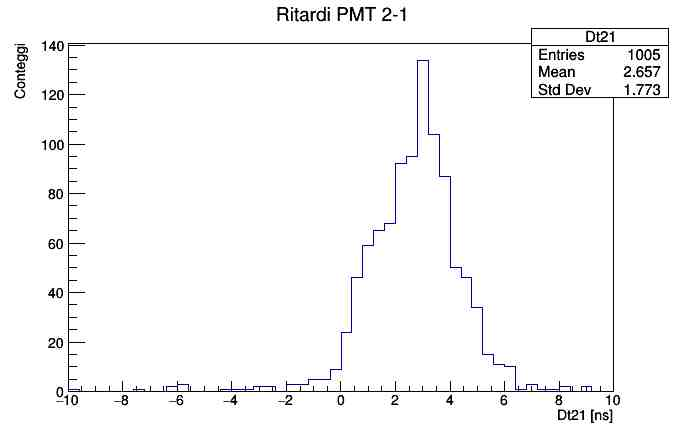
\includegraphics[width=\textwidth]{./immagini/TimeOfFlight/Rit21Fore.jpg}
         \caption{}
         \label{fig:Dt21ForeA}
     \end{subfigure}
     \hfill
     \begin{subfigure}[b]{0.4\textwidth}
         \centering
         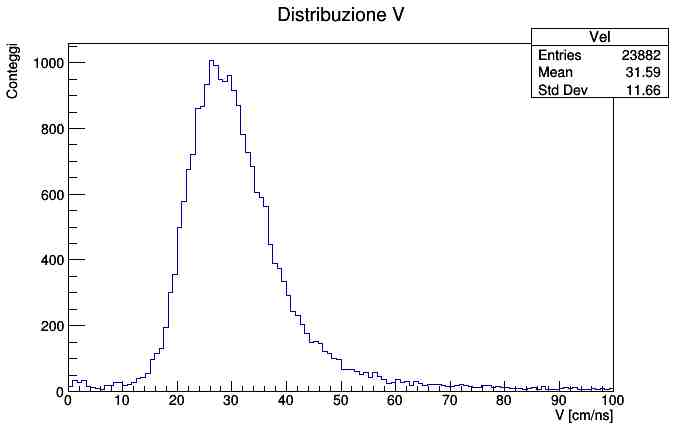
\includegraphics[width=\textwidth]{./immagini/TimeOfFlight/VFore.jpg}
         \caption{}
         \label{fig:VForeA}
     \end{subfigure}
     \end{center}
     \caption{Per fare queste misure i time stamp sono stati valutati prendendo il baricentro della discesa negativa del segnale, considerando, quindi, come inizio l'inizio del segnale meno un'unità di tempo, mentre come fine il minimo del segnale più 3 campioni.}        
     \label{fig:ForeA}
\end{figure}

\begin{table}[H]
\begin{tabular}{c|c|c}
$R_{21}$ [ns] & $R_{31}$ [ns] & $R_{32}$ [ns] \\
\hfill
2,74 $\pm$ 1,42 & -10,0 $\pm$ 1,48 & -12,8 $\pm$ 1.65
\hfill
\end{tabular}
\caption{}
\label{tab:RitForeA}
\end{table}

Dal confronto con le altre prove questo tentativo ha una devstd minore sia sul ritardo $R_{21}$ che sulla distribuzione di V.

\subsection{Scelta calcolo time-stamp}
\label{sec:AScelta}
La scelta tra i vari metodi di calcolo del time-stamp è stata fatta considerando i risultati ottenuti tramite fit delle distribuzioni dei ritardi tra i PMT e la relativa ricostruzione della distribuzione di V.\\
\'E stato scelto di utilizzare il metodo tramite integrazione di una parte più ampia della sola discesa del segnale (l'ultimo tentativo), in particolare 4\,ns (1 campione dell'adc) prima dell'inizio del segnale e 12\,ns dopo il minimo di esso (3 campioni oltre).\\
In questa maniera, oltre che rimanere il più possibile fedeli alla definizione di time-stamp, si considera una parte di segnale che a meno di ampiezze differenti rimane molto simile tra i vari segnali.\\
Inoltre, si potrebbero mediare eventuali problemi di ricostruzione del picco e non considerare alcuni fastidiosi ringing, che può presentare il segnale.\\
Come ultima osservazione i risultati ottenuti hanno tutti una devstd minore, il che porta a pensare che potrebbe essere la misura più accurata.

\section{Codice Python}
\label{sec:ARep}
Ho inserito un repositorio online al link:
\begin{center}
\url{https://github.com/AndreaForesi/LabIntFon20-21.git}
\end{center}
Il codice di analisi dati è scritto quasi interamente su Python.\\
I fit sugli scatterplot e altri grafici sono stati riprodotti utilizzando Matlab o Root-Cern.

\end{document}